\documentclass[conference]{IEEEtran}
\usepackage{fontspec}
\setmainfont{texgyretermes}[Extension=.otf, UprightFont=*-regular,
  BoldFont=*-bold, ItalicFont=*-italic, BoldItalicFont=*-bolditalic]
\usepackage{graphicx}
\usepackage{amsmath}
\usepackage{array}
\usepackage{xcolor}
% hyperref loads last so its patches of \ref, \label and \cite win.
\usepackage{hyperref}
\hypersetup{
  colorlinks=true,
  linkcolor=blue!60!black,
  citecolor=green!40!black,
  urlcolor=blue!60!black,
  pdftitle={Frequent Itemset Mining with Eclat and Two Applications},
  pdfauthor={Hung, Thien, Phat},
}
% Rows of the optimization-step table get labels so prose cites them with \ref.
\newcounter{optstep}
\newcommand{\optstep}[1]{\refstepcounter{optstep}\theoptstep\label{#1}}
\title{Frequent Itemset Mining with Eclat and Two Applications}
\author{\IEEEauthorblockN{Hung \and Thien \and Phat}
\IEEEauthorblockA{University of Science, VNU-HCM}}
\begin{document}
\maketitle
\begin{abstract}
We implement Zaki's Eclat algorithm in Julia using only the standard library, evaluate
it on five benchmark databases, and apply it to two practical problems. The package
contains a baseline that stays close to the original paper and an optimized variant that
adds bitset tidsets, a search order by increasing support, perfect-extension pruning,
pair counting, and tid lists for sparse data. Both variants match SPMF's Eclat exactly at
every database and threshold we tested. On the grading machine, the optimized variant is
the fastest of four programs (our two variants, SPMF Eclat, and SPMF PrePost+) at all 33
points, and at the lowest minsup of each database it runs 7.9 to 33.3 times faster than
the baseline. When the transaction length grows from 5 to 40 with the output size held
fixed, the baseline's mining time grows 42-fold, while the optimized variant's grows only
1.8-fold. We apply the miner to market basket analysis on Online Retail II and to
image-pattern mining on Semeion.
\end{abstract}
\section{Introduction}
Frequent itemset mining (FIM) finds the sets of items that occur together in at least
$\sigma_{\min}$ transactions of a database, where $\sigma_{\min}$ is the minimum support
threshold (called minsup when written as a fraction of the database). It is the first
step of association rule mining and underlies many other pattern-mining tasks. Because
the number of frequent itemsets can grow very quickly as the threshold drops, the way an
algorithm lays out the data and counts support decides how low a threshold it can reach.

Eclat~\cite{zaki2000} stores the database vertically, pairing each item with its tidset,
the set of identifiers of the transactions that contain it. The support of an itemset is
then the size of the intersection of its items' tidsets, and Eclat searches depth-first
over prefix-based equivalence classes. We reimplemented the algorithm from the original
paper in Julia using only the standard library, compared it with SPMF's Eclat and
PrePost+~\cite{spmf2016}, and used it in two applications. The rest of the paper is
organized in three parts:
\begin{itemize}
\item Section~\ref{sec:implementation} presents a baseline that follows the paper and an
optimized variant (bitsets, a search order by increasing support, perfect-extension
pruning, pair counting, and tid lists for sparse data), together with a correctness
argument, the test suite, and the measured gain of each optimization.
\item Section~\ref{sec:evaluation} describes the shared measurement protocol
(Section~\ref{sec:protocol}), checks every itemset against SPMF
(Section~\ref{sec:exact}), and reports runtime against minsup
(Section~\ref{sec:minsup}), the number of frequent itemsets against minsup
(Section~\ref{sec:output-size}), peak memory (Section~\ref{sec:memory}), scalability
with database size (Section~\ref{sec:scalability}), the effect of transaction length
(Section~\ref{sec:width}), and two directions for further optimization
(Section~\ref{sec:future}).
\item Section~\ref{sec:applications} applies Eclat to market basket analysis on Online
Retail II (Section~\ref{sec:basket}) and to image-pattern mining on Semeion
(Section~\ref{sec:visual-patterns}).
\end{itemize}

We follow two rules when presenting results. First, a performance comparison only uses
runs whose output, both itemsets and supports, matches an independent run of SPMF's
Eclat exactly, since two programs can report the same number of itemsets with different
supports. Second, every headline number is tied to the machine and the source revision
that produced it, and every random step uses seed 42. The project repository contains the
source code, configurations, data hashes, and reproduction commands for every experiment.

\section{Implementation}
\label{sec:implementation}
We reimplemented Eclat from Zaki's original paper~\cite{zaki2000} in Julia, using only
the standard library and no frequent itemset mining (FIM) library. The package has two
variants that return the same result: a baseline that follows the paper closely, and an
optimized variant. This section explains the algorithm and why it is correct, how we test
it, which optimizations we added, and how much each one improved on the baseline.

\subsection{Vertical layout and tidsets}
A database holds $N$ transactions. Each transaction gets a transaction identifier (tid),
the index $1, 2, \dots, N$ in the order it is read. Apriori stores the database in a
horizontal layout, where each transaction carries its list of items. Eclat uses a
vertical layout, where each item $x$ carries its tidset $t(x)$, the set of tids of the
transactions that contain $x$. For an itemset $X$,
\begin{equation}
  t(X) = \{\, i \in \{1,\dots,N\} : X \subseteq T_i \,\}, \qquad
  \sigma(X) = |t(X)|,
  \label{eq:support}
\end{equation}
where $T_i$ is the $i$-th transaction and $\sigma(X)$ is the support of $X$, the number
of transactions that contain $X$. An itemset $X$ is frequent when
$\sigma(X) \ge \mathit{minsup}$, with $\mathit{minsup}$ the minimum support threshold
counted in transactions. An empty transaction still has a tid and still counts toward
$N$, but it appears in no tidset.

The baseline stores each tidset as an increasing \texttt{Vector\{Int\}}, called a
tid-list. The function \texttt{to\_class} reads the database once and appends tids in
increasing order, so every tid-list is already sorted and never needs sorting again.

The main advantage of the vertical layout is the intersection. A transaction contains
$P \cup \{a, b\}$ if and only if it contains both $P \cup \{a\}$ and $P \cup \{b\}$, so
\begin{equation}
  t(P \cup \{a, b\}) = t(P \cup \{a\}) \cap t(P \cup \{b\}),
  \label{eq:intersect}
\end{equation}
where $P$ is an itemset and $a, b$ are two items not in $P$. The support of the new
itemset therefore comes from two tidsets that already exist, without another scan of the
database.

\subsection{Prefix-based equivalence classes and Bottom-Up search}
Zaki partitions the search space into prefix-based equivalence
classes~\cite{zaki2000}. The class with prefix $P$ holds the members
$(b, t(P \cup \{b\}))$, one for each item $b$ greater than every item of $P$. Two itemsets
in the same class differ only in their last item, so intersection~\eqref{eq:intersect}
is valid only between members of the same class.

The function \texttt{bottom\_up!} implements the paper's Bottom-Up procedure. For each
member $a$ of the class with prefix $P$, it records $P \cup \{a\}$ and its support,
intersects $t(P \cup \{a\})$ with the tidset of every member $b$ after $a$, keeps the
frequent results as the child class with prefix $P \cup \{a\}$, and searches that child
class before moving to the next member. The root class has the empty prefix and holds the
frequent items. The paper allows a depth-first search (DFS) or a breadth-first search over
the lattice of classes and reports results breadth-first. We chose depth-first so that
memory holds only one class per level of the current path. The paper also counts the
frequent 2-itemsets in advance with a triangular array over the horizontal database. The
baseline starts intersecting from single items so that one procedure handles every
level, and the optimized variant brings this counting step back in
Section~\ref{sec:optimized}. Table~\ref{tab:mapping} maps the parts of the paper to the
source code.

\begin{table}[t]
\centering
\small
\caption{Mapping from the paper~\cite{zaki2000} to the source code in \texttt{src/algorithm/}}
\label{tab:mapping}
\begin{tabular}{>{\raggedright\arraybackslash}p{0.37\columnwidth}>{\raggedright\arraybackslash}p{0.53\columnwidth}}
\hline
Paper & Baseline; optimized variant \\
\hline
Item tid-lists (Section 4.1) & \texttt{to\_class}; \texttt{bitset\_tidsets} \\
Prefix classes (Section 4.2) & vector of (item, tid-list) pairs; vector of
\texttt{ClassMember\{T\}} \\
Bottom-Up (Sections 4.3.1 and 5.2, Fig.~12) & \texttt{bottom\_up!}; \texttt{eclat\_search!} \\
Intersecting two tid-lists & \texttt{intersect\_tidlists}; \texttt{intersect\_bitsets!} and
\texttt{intersect\_lists!} \\
Counting 2-itemsets with a triangular array (Section 5.1) & not used; \texttt{count\_pairs} \\
\hline
\end{tabular}
\end{table}

Table~\ref{tab:trace} traces the algorithm on the database \texttt{baskets.txt}, which has
four transactions $T_1 = \{1,2,3\}$, $T_2 = \{1,2\}$, $T_3 = \{1,3\}$, $T_4 = \{2,3\}$,
with $\mathit{minsup} = 2$. The initial tidsets are $t(1) = \{1,2,3\}$,
$t(2) = \{1,2,4\}$, and $t(3) = \{1,3,4\}$. The algorithm records exactly six frequent
itemsets, and it prunes $\{1,2,3\}$ because only $T_1$ contains it.

\begin{table}[t]
\centering
\caption{Bottom-Up trace on \texttt{baskets.txt} with $\mathit{minsup} = 2$}
\label{tab:trace}
\begin{tabular}{llll}
\hline
Prefix & Intersection & Tidset & Result \\
\hline
$\emptyset$ & -- & $t(1) = \{1,2,3\}$ & record $\{1\}$, $\sigma = 3$ \\
$\{1\}$ & $t(1) \cap t(2)$ & $\{1,2\}$ & keep $2$ \\
$\{1\}$ & $t(1) \cap t(3)$ & $\{1,3\}$ & keep $3$ \\
$\{1\}$ & -- & $t(12) = \{1,2\}$ & record $\{1,2\}$, $\sigma = 2$ \\
$\{1,2\}$ & $t(12) \cap t(13)$ & $\{1\}$ & prune, $1 < 2$ \\
$\{1\}$ & -- & $t(13) = \{1,3\}$ & record $\{1,3\}$, $\sigma = 2$ \\
$\emptyset$ & -- & $t(2) = \{1,2,4\}$ & record $\{2\}$, $\sigma = 3$ \\
$\{2\}$ & $t(2) \cap t(3)$ & $\{1,4\}$ & keep $3$ \\
$\{2\}$ & -- & $t(23) = \{1,4\}$ & record $\{2,3\}$, $\sigma = 2$ \\
$\emptyset$ & -- & $t(3) = \{1,3,4\}$ & record $\{3\}$, $\sigma = 3$ \\
\hline
\end{tabular}
\end{table}

\subsection{Correctness}
\label{sec:correctness}
Every class that \texttt{bottom\_up!} receives satisfies four invariants: (i) each
tid-list is increasing and has no duplicates; (ii) the members are sorted by item and
every member item is greater than every item of the prefix; (iii) every member is
frequent; (iv) the tid-list of member $b$ equals $t(P \cup \{b\})$. The root class
satisfies all four when it is built. A child class takes the members after $a$, so it
keeps (i) and (ii). The size check before a member is added gives (iii), and
identity~\eqref{eq:intersect} gives (iv).

Three properties follow. First, every recorded support is exact, by (iv)
and~\eqref{eq:support}. Second, no itemset is recorded twice: by (ii) every key
$(x_1, \dots, x_k)$ is strictly increasing, and it is recorded only when the class with
prefix $(x_1, \dots, x_{k-1})$ reaches $x_k$, and each class is built only once. Third,
the result is complete because support is anti-monotone: if $X \subseteq Y$ then
$\sigma(X) \ge \sigma(Y)$, so pruning an infrequent itemset never loses a frequent
superset. Induction on length shows that the class with prefix $(x_1, \dots, x_{j-1})$
contains every item $y > x_{j-1}$ for which $(x_1, \dots, x_{j-1}, y)$ is frequent, so
every frequent itemset is recorded. The repository file \texttt{docs/eclat.md} gives the
full proof.

\subsection{Complexity}
Let $L$ be the total number of items over all transactions, $m$ the number of distinct
items, and $C$ the number of intersections. Building the vertical layout takes $O(L)$
expected time for the dictionary, $O(m \log m)$ for sorting, and $O(L)$ memory. One
intersection costs $O(|t(P \cup \{a\})| + |t(P \cup \{b\})|)$, at most $O(N)$. A class
with $k$ members performs $k(k-1)/2$ intersections, so the total time is
\begin{equation}
  O(L + m \log m + C \cdot N),
  \label{eq:cost}
\end{equation}
where $C$ is the total number of intersections over all classes visited. Because the
search is depth-first, memory holds only the classes on the current path, one class per
level, each with at most $m$ members of at most $N$ tids. The output can grow
exponentially: a frequent $k$-itemset has $2^k - 1$ non-empty subsets, and all of them
are frequent.

\subsection{Interface, SPMF format, and command line}
The two applications and the experiments call only four public functions.
\texttt{read\_transactions} reads an SPMF file (one transaction per line, items separated
by spaces). \texttt{support\_threshold} converts $\mathit{minsup}$ to a transaction
count. \texttt{mine} returns a \texttt{SupportMap} dictionary from itemset to support.
\texttt{write\_itemsets} writes one itemset per line in the form
\texttt{1 2 \#SUP: 2}. A real $\mathit{minsup}$ in $(0, 1]$ is a fraction and is
rounded up to $\lceil \mathit{minsup} \cdot N \rceil$ transactions; an integer
$\mathit{minsup}$ is an absolute transaction count. The \texttt{variant} argument
selects \texttt{:baseline} or \texttt{:optimized}, so each variant can be run on its own
and compared on the same input.

The command-line program \texttt{demo.jl} takes an input path, \texttt{--output},
exactly one of the two thresholds \texttt{--minsup} (a fraction) or
\texttt{--min-count} (a transaction count), and \texttt{--variant}, for example
\texttt{julia --project=. demo.jl --minsup 0.5 --output out.txt data/toy/baskets.txt}.
Invalid input stops the program with exit code 1 and a message that names the offending
line. The writer validates the whole result before it opens the file, so a failed run
leaves an existing output file untouched. Itemsets are written in lexicographic order of
their item codes, so the output files of the two variants are identical byte for byte.

\subsection{Automated tests}
\label{sec:tests}
The command \texttt{julia --project=. test/runtests.jl} runs 1\,091 checks, and all of
them pass on Julia 1.13.2. Each mining test compares the whole \texttt{SupportMap} and
also the number of itemsets recorded, because the dictionary would hide an itemset
recorded twice. Both variants run the following groups of tests.

\begin{itemize}
\item Hand-derived results: eight small databases, including an empty database, a
database with no frequent itemset, duplicate transactions, thresholds just above and
just below an itemset's support, and an image database with empty transactions.
\item Comparison with SPMF's Eclat~\cite{spmf2016}: eight runs on seven small databases
and one run on T25I10D10K (9\,976 transactions, 929 items), where SPMF reports 14\,782
itemsets of 1 to 13 items at $\mathit{minsup} = 0.008$. Both variants match 100\% on all
nine runs, with no missing, extra, or wrong-support itemset.
\item Comparison with a brute-force counter that enumerates every subset: 10 random
databases generated with seed 42 for each variant. The optimized variant also runs eight
databases with 0, 1, 63, 64, 65, 127, 128, and 129 transactions, which sit around the
boundary of one 64-bit bitset word. Half of them contain groups of items that always
occur together, to produce perfect extensions. Each database runs under 18
configurations that switch each technique of Section~\ref{sec:optimized} on and off.
\item Type stability: \texttt{Test.@inferred} on \texttt{mine}, \texttt{mine\_packed},
and the search functions of both variants.
\item Reading, writing, and the command line: the byte-level reader is checked against a
line-based parser on edge-case inputs (\texttt{Int} overflow, unexpected characters,
blank lines, Windows line endings) and on every small database. The writer is compared
byte for byte with a reference formatter, and argument errors and process exit codes are
checked.
\end{itemize}

The brute-force counter is only a test tool. Outside the test suite, every measurement
campaign in Section~\ref{sec:measure} compares each output file with an independent run
of SPMF's Eclat after timing ends. The final campaign produced 820 output files on the
five benchmark databases (615 from the optimized variant and 205 from PrePost+), and all
820 match 100\%.

\subsection{Optimized variant}
\label{sec:optimized}
The optimized variant keeps the Bottom-Up procedure and changes three things: how
tidsets are stored, which intersections are skipped, and how the result is written. Each
change keeps the output exact, and the proofs are in \texttt{docs/eclat-optimized.md}.
Start-up, reading, and writing live in shared code, so both variants benefit from the
changes there.

\subsubsection{Bitset tidsets and search order}
At the lowest threshold of each database, the baseline's mining call allocates 3.3 to
5.7 GiB, mostly for the new tid-list of each intersection. The optimized variant stores
each tidset as a bitset, a bit string in which bit $i$ stands for transaction $i$, made of
$W = \lceil N/64 \rceil$ 64-bit words. An intersection is a word-by-word AND, and the
support is the number of set bits, counted with \texttt{count\_ones} in the same loop.
The result goes into a bitset taken from a reusable pool. The bitset of an infrequent
intersection goes back to the pool, so a failed intersection allocates no memory. An
intersection reads $2W$ words whatever the support: $W = 50$ on Chess and $5\,316$ on
Accidents.

Items are visited in increasing order of support. The rare item that comes first is
intersected with the most items, but most of those intersections fail, and the frequent
item that comes last has few members after it, so child classes are smaller. The proof
in Section~\ref{sec:correctness} only needs a total order on the items, so it holds for
this order too.

\subsubsection{Perfect-extension pruning and single allocation of the result}
An item $b$ is a perfect extension~\cite{borgelt2012} of an itemset $X$ when
$t(X \cup \{b\}) = t(X)$, that is, when every transaction that contains $X$ also contains
$b$. Since $t(X \cup \{b\}) \subseteq t(X)$, the condition is equivalent to the two
supports being equal, so a single count comparison decides it. Every itemset $X \cup Y$
in the subtree of $X$ then has the same support as $X \cup Y \cup S$, where $S$ is any
subset of the set $E$ of perfect extensions. The optimized variant therefore removes $b$
from the child class and never intersects $b$'s tidset again. Each node of the search
tree stands for $2^{|E|}$ itemsets with the same support. On Mushroom 0.05 the search tree
has only 33\,819 nodes for 3\,755\,511 itemsets.

The search records only the nodes, in preorder. Each node holds its depth, the item it
adds, the perfect extensions it found, and its support. The function
\texttt{expand\_nodes} computes the final size of the result from the nodes, with an
overflow check, allocates the three result arrays exactly once, and then writes the
subsets $S$ in Gray-code order, so that two consecutive itemsets differ by one item. If
the result arrays grow one itemset at a time, each doubling of capacity copies the whole
array. On Mushroom 0.05, the mining call in an already warm process allocated 1\,068 MiB
to build a 306 MiB result and took 0.40 s. With a single allocation it allocates 310 MiB
and takes 0.17 s.

\subsubsection{Sparse data: pair counting, tid lists, and block bounds}
On sparse data, a bitset intersection still reads all $W$ words even when the tidsets are
short ($W = 1\,378$ on Retail and $1\,563$ on T10I4D100K), and most intersections fail.
On Retail 0.001, 99.9\% of the 2\,239\,786 intersections in the root class miss the
threshold. On T10I4D100K 0.00025, most intersections happen at depth 2 (2\,256\,822 of
them, 99.1\% failing) on tidsets of only about 100 tids. Three techniques address these
two patterns.

\emph{Pair counting at the root.} The function \texttt{count\_pairs} counts the support
of every pair of frequent items in a triangular array of $m_f(m_f-1)/2$ cells during one
pass over the horizontal database, as in Section 5.1 of the paper~\cite{zaki2000}, where
$m_f$ is the number of frequent items. The root class intersects only the pairs that
reach the threshold. At the root the prefix is empty, so the count of pair $(a, b)$ is
exactly $|t(\{a, b\})|$ and no frequent intersection is skipped. The counting runs only
when its estimated cost is below one tenth of the cost of the root intersections, that
is, when $10 \sum_i |T_i|(|T_i| - 1)/2 < W m_f(m_f-1)/2$. Retail and T10I4D100K meet this
condition. Chess, Mushroom, and Accidents, with long transactions and few frequent items,
intersect at the root as before.

\emph{Per-class tid lists.} A child class with $k$ members switches from bitsets to
increasing tid lists when
\begin{equation}
  kW + c\,(k - 1) \sum_{i=1}^{k} \sigma_i < W\,\frac{k(k-1)}{2},
  \label{eq:lists}
\end{equation}
where the right-hand side is the number of words the class's bitset intersections would
read, $kW$ is the cost of the conversion, $\sigma_i$ is the support of the $i$-th
member, and $c = 8$ is the cost of one merge step in words, chosen from a sweep of $c$
from 2 to 16 on the measurement machine. Rule~\eqref{eq:lists} depends on tidset lengths
and $N$, not on the name of the database. The merge of two lists has no data-dependent
branches, and it stops early once the common tids found so far plus the rest of the
shorter list cannot reach $\mathit{minsup}$.

\emph{Block bounds.} On T10I4D100K 0.00025, 98.7\% of the 2\,076\,972 merges still fail,
on two lists that hold 126 tids between them on average. Before it searches a class of
tid lists, the program splits the tid range into at most $K = 256$ blocks whose width is a
power of two, and counts the tids of each member in each block. For two members $X$ and
$Y$ of the class,
\begin{equation}
  \sigma(X \cup Y) \le \sum_{j=1}^{K} \min(c_{X,j}, c_{Y,j}),
  \label{eq:bound}
\end{equation}
where $c_{X,j}$ and $c_{Y,j}$ are the numbers of tids of $X$ and $Y$ in block $j$,
because a common tid lies in exactly one block and is counted once for each member. A
merge whose bound is below $\mathit{minsup}$ is skipped without reading any tid.
Bound~\eqref{eq:bound} never rejects a frequent intersection, so the output does not
change. We chose $K = 256$ from a sweep of 64 to 512 blocks.

\subsubsection{Start-up, reading, and writing}
The changes in this subsection are in the code shared by both variants. At high
thresholds, the runtime is not spent in the algorithm. One \texttt{demo.jl} process of
the baseline on Chess 0.9 takes 2.36 s, while Julia start-up takes only 0.17 s. The rest
is just-in-time (JIT) compilation. We run the public functions and the command-line
handling on a small database while Julia builds the package image, so their machine code
is stored with the package. The command-line handling lives in the package
(\texttt{src/cli.jl}) and not in the script file, because script code is not stored in
the package image and would be recompiled for 108.6 ms on every run. A test runs
\texttt{demo.jl} in a fresh process with \texttt{--trace-compile} and requires that no
method needs compiling.

At low thresholds on dense data, most of the time goes into writing the result. The
\texttt{Profile} sampler on Mushroom 0.05 showed that the comparison sort of the output
took 64\% of the time, formatting and writing the file 25\%, and mining only 11\%. The
optimized variant visits items by support, so it has to sort the result back into
lexicographic order. We replaced that sort with a radix sort on a 128-bit key that holds
the first items of the itemset and its index. The writer takes the digits of every number
below $2^{20}$ from a lookup table and writes them with one 8-byte store. The reader parses
each line into a reused vector and copies it once at its final length, so reading
Accidents (34 MB) in a warm process dropped from 0.57 s to 0.29 s and allocates 151 MiB
instead of 354 MiB.

\subsubsection{Julia features}
The type \texttt{ClassMember\{T\}} has a parameter \texttt{T}, which is \texttt{UInt64}
for bitsets or \texttt{Int} for tid lists. The search function \texttt{eclat\_search!}
is written once, and multiple dispatch (choosing a method from the types of all
arguments) picks the intersection, the conversion rule, and the intersection filter from
\texttt{T}. Julia compiles a specialized version for each tidset form, so the inner loop
has no run-time type checks. We use \texttt{Vector\{UInt64\}} instead of
\texttt{BitVector} because the intersection loop writes into reused memory and counts
bits in the same pass.

The key type \texttt{Tuple\{Vararg\{Int\}\}} of \texttt{SupportMap} has no fixed length,
so building millions of keys costs more than mining itself. In an early test on
Mushroom 0.05, inserting 3.76 million itemsets into the dictionary took 12.4 s, while
counting their supports took 0.63 s. Both variants therefore write their result into
three flat \texttt{Vector\{Int\}} arrays (the items, the start position of each itemset,
and the supports). The file writer reads these arrays directly, and \texttt{mine} builds
a \texttt{SupportMap} only at the interface boundary for the applications. Every tuning
constant is \texttt{const}, and every container on a hot path has a concrete element type.
\texttt{@inbounds} appears only in the tid-list merge and the number writer, with a
comment that proves the indices valid. On the bitset intersection loop,
\texttt{@inbounds @simd} changed mining time by $-8\%$ to $+11\%$ over five measurement
points, which is within noise, so we do not use it.

\subsection{Measuring the improvement}
\label{sec:measure}
Every number in this subsection is the median time of five cold \texttt{demo.jl}
processes: each run is a fresh process that includes Julia start-up, reading, mining, and
writing the file. The campaigns ran on a Linux machine (Intel Core i7-11800H, 7.4 GiB
RAM, clock fixed at 2.3 GHz) with single-threaded Julia 1.13.2. The grid has 33
thresholds on the five databases Chess, Mushroom, Retail, T10I4D100K, and Accidents,
plus some stress thresholds below the grid that only probe the limits. Besides SPMF's
Eclat, we compare with PrePost+~\cite{deng2015} from the
\href{https://github.com/NgTHung/Itemset/blob/main/tools/spmf/release.toml}{pinned SPMF release}
(Java Temurin 25.0.4.1, 4 GiB heap), because it is faster than SPMF's Eclat on dense
data. The ratio $R = T_\text{opt} / T_\text{PrePost+}$ divides the median time of the
optimized variant by the median time of PrePost+ at the same threshold.

Each technique was measured in its own session, in which the versions before and after
the change alternate on every repeat, so machine drift affects both equally. Only the
precompilation step was measured as two consecutive campaigns. Table~\ref{tab:steps} gives
the after-over-before time ratio of each step over the 33 thresholds, and the matching
peak-memory ratio. Peak memory is the peak resident set size (RSS), the largest amount of
physical memory the process holds, as measured by the operating system.

\begin{table*}[t]
\centering
\small
\caption{Effect of each optimization step over 33 thresholds: after-over-before ratios of
time and peak memory (below 1 is better), and the threshold that improved most}
\label{tab:steps}
\begin{tabular}{rllll}
\hline
Step & Technique & Time ratio & Example, time before $\to$ after (s) & Memory ratio \\
\hline
\optstep{step:precompile-package} & Precompile the package functions & 0.14 to 0.83 & Chess 0.9: 2.36 $\to$ 0.33 & 0.82 to 0.97 \\
\optstep{step:bitset} & Bitsets and increasing-support order & 0.10 to 0.97 & Mushroom 0.1: 6.28 $\to$ 0.88 & 0.68 to 0.99 \\
\optstep{step:perfect-extension} & Perfect-extension pruning & 0.93 to 1.04 & Mushroom 0.1: 0.89 $\to$ 0.83 & 0.95 to 1.00 \\
\optstep{step:radix-sort} & Radix sort for output order & 0.77 to 1.02 & Mushroom 0.1: 0.83 $\to$ 0.64 & 1.00 to 1.02 \\
\optstep{step:precompile-cli} & Precompile the command line & 0.66 to 0.94 & Chess 0.9: 0.33 $\to$ 0.22 & 0.91 to 1.03 \\
\optstep{step:pair-count} & Pair counting at the root & 0.24 to 1.01 & Retail 0.001: 1.72 $\to$ 0.42 & 1.00 to 1.03 \\
\optstep{step:tid-lists} & Per-class tid lists & 0.83 to 1.02 & T10I4D100K 0.00025: 1.46 $\to$ 1.21 & 1.00 to 1.01 \\
\optstep{step:byte-io} & Byte-level reading and writing, digit table & 0.76 to 0.99 & Accidents 0.65: 1.10 $\to$ 0.85 & 0.74 to 1.00 \\
\optstep{step:single-allocation} & Single result allocation, block bounds & 0.82 to 1.03 & T10I4D100K 0.00025: 1.18 $\to$ 0.97 & 0.83 to 1.02 \\
\hline
\end{tabular}
\end{table*}

Step~\ref{step:bitset} has the largest effect: time drops to 10\% to 97\% of the baseline
(median 37\%), and peak memory falls at every threshold. Step~\ref{step:pair-count} only
affects sparse data, where it cuts the time of Retail 0.001 by 76\%.
Step~\ref{step:perfect-extension} on its own shortens process time by at most 6.9\%,
because at that threshold sorting and writing hundreds of thousands of itemsets takes
most of the time. We keep it because it does not raise memory and because
step~\ref{step:single-allocation} builds on it. No step slows any threshold by more than
4.4\%.

Table~\ref{tab:final} shows the combined effect of steps~\ref{step:bitset}
to~\ref{step:single-allocation} at the highest and lowest threshold of each database. It
compares the baseline after step~\ref{step:precompile-package} with the optimized variant
after step~\ref{step:single-allocation}. Steps~\ref{step:precompile-cli}
and~\ref{step:byte-io} are in shared code, so the baseline of the submitted version also
benefits from them; the comparison of the two variants on the same code version is
step~\ref{step:bitset} of Table~\ref{tab:steps}. The two columns were measured in two
sessions three days apart on the same machine and configuration. PrePost+ ran in both
sessions, and its median differed between them by $-3.8\%$ to $+5.8\%$ (median
$+0.3\%$), so the two sessions are comparable within that margin.

\begin{table*}[t]
\centering
\small
\caption{Median cold process time (s) and maximum peak memory (MiB) over five runs. The
baseline (after step~\ref{step:precompile-package}) was measured on 2026-11-06, the
optimized variant (after step~\ref{step:single-allocation}) and PrePost+ on 2026-11-09,
and SPMF's Eclat on 2026-10-31, all on the same machine}
\label{tab:final}
\begin{tabular}{lrrrrrrrr}
\hline
 & & \multicolumn{5}{c}{Time (s)} & \multicolumn{2}{c}{Peak memory (MiB)} \\
Data / minsup & Itemsets & Baseline & Optimized & Speedup & SPMF Eclat & PrePost+ & Baseline & Optimized \\
\hline
Chess / 0.9 & 622 & 0.33 & 0.21 & 1.6 & 0.51 & 0.42 & 268 & $\le 254$ \\
Chess / 0.6 & 254\,944 & 3.24 & 0.30 & 10.8 & 15.98 & 0.59 & 308 & 262 \\
Mushroom / 0.5 & 153 & 0.33 & 0.22 & 1.5 & 0.51 & 0.44 & 256 & $\le 254$ \\
Mushroom / 0.1 & 574\,431 & 6.28 & 0.40 & 15.7 & 7.44 & 0.68 & 414 & 302 \\
Retail / 0.01 & 159 & 0.55 & 0.29 & 1.9 & 1.19 & 0.80 & 304 & $\le 254$ \\
Retail / 0.001 & 7\,589 & 12.80 & 0.38 & 33.5 & 1.53 & 3.52 & 331 & 281 \\
T10I4D100K / 0.01 & 385 & 2.93 & 0.32 & 9.1 & 0.78 & 1.42 & 304 & $\le 254$ \\
T10I4D100K / 0.00025 & 96\,959 & 10.92 & 0.97 & 11.3 & 8.02 & 4.34 & 363 & 279 \\
Accidents / 0.95 & 15 & 1.31 & 0.78 & 1.7 & 4.59 & 1.71 & 650 & 397 \\
Accidents / 0.65 & 1\,093 & 7.13 & 0.86 & 8.3 & 26.87 & 2.34 & 804 & 397 \\
\hline
\end{tabular}
\end{table*}

Across all 33 thresholds, steps~\ref{step:bitset} to~\ref{step:single-allocation} shorten
process time by 1.5 to 33.5 times (median 4.0). The geometric mean speedup per database is
3.1 on Accidents, 3.3 on Mushroom, 3.4 on Chess, 6.5 on Retail, and 13.5 on T10I4D100K.
The smallest gains are at the high thresholds of Chess and Mushroom, where a run takes
only about 0.22 s, of which 0.19 s is Julia start-up and package loading. Most of the gain
there comes from step~\ref{step:precompile-cli}. Against SPMF, the optimized variant is
2.3 to 53 times faster than Eclat, using the Eclat measurements from the 2026-10-31
session, and faster than PrePost+ at all 33 thresholds, with $R$ from 0.11 to 0.59. The
geometric mean of $R$ per database is 0.20 on Retail, 0.21 on T10I4D100K, 0.41 on
Accidents, 0.49 on Mushroom, and 0.51 on Chess. The interquartile range (IQR) of the
Baseline and Optimized columns stays within 3.3\% of the median at every threshold.

After step~\ref{step:single-allocation}, peak memory is lower than the baseline's at
every threshold. The largest drop is on Accidents (804 to 397 MiB at 0.65), because the
reader no longer over-allocates and the tidsets take only a few MiB during the search. On
the measurement machine, all three programs (Julia, SPMF Eclat, and PrePost+) report
their lowest values between 253.0 and 253.6 MiB, so the measurement has a common floor,
and the cells marked $\le 254$ in Table~\ref{tab:final} are only upper bounds.

We tried, measured, and dropped three techniques. Diffsets~\cite{zaki2003} store the tids
that a member lacks relative to its prefix. In a sweep of the switching ratio, no value
was faster than bitsets: Accidents 0.2 slowed by up to 10\% and T10I4D100K 0.00025 by up
to 71\%. The reason is that perfect-extension pruning already removes every member with
an empty diffset, which is exactly where diffsets help most. Even with the best choice for
each class, the number of words read dropped by at most 0.3\%. Printing itemsets directly
from the sort key was 5\% to 7\% slower. The \texttt{@inbounds @simd} annotation on the
bitset intersection gave no improvement beyond noise.

The optimized variant has three measured limits. First, at the stress threshold
Mushroom 0.05, the program has to write 3\,755\,511 lines and remains slower than
PrePost+ (1.45 s against 1.38 s). Second, each process spends about 0.19 s on Julia
start-up and package loading, which could only be removed by compiling the whole program
ahead of time into an executable. Third, pair counting raises peak memory by 20\% at the
stress threshold Retail 0.00025, because the triangular array for 5\,918 frequent items
takes 67 MiB.

\section{Experiments and evaluation}
\label{sec:evaluation}
\subsection{Data and shared protocol}
\label{sec:protocol}
We ran the experiments on five standard benchmark databases from the FIM community:
Chess, Mushroom, Retail, T10I4D100K, and Accidents, all originally from the FIMI
repository~\cite{fimi}. Table~\ref{tab:datasets} lists statistics that we computed from
the data files themselves, where $N$ is the number of transactions, $|I|$ the number of
distinct items, $\bar{w}$ the mean transaction length, and the density
$d = \bar{w} / |I|$ the average fraction of items present in a transaction. Chess and
Mushroom are dense ($d \ge 0.19$), while Retail and T10I4D100K are sparse
($d \le 0.012$). Accidents has $d = 0.072$, between the two groups, but we group it with
the dense databases because of its long transactions ($\bar{w} = 33.81$, close to Chess),
which make its output grow as fast as theirs (Section~\ref{sec:output-size}).

\begin{table}[t]
\centering
\caption{Statistics of the five benchmarks, computed from SHA-256-checked files}
\label{tab:datasets}
\begin{tabular}{lrrrrr}
\hline
Data & $N$ & $|I|$ & $\bar{w}$ & $w_{\max}$ & $d$ \\
\hline
Chess & 3\,196 & 75 & 37.00 & 37 & 0.493 \\
Mushroom & 8\,124 & 119 & 23.00 & 23 & 0.193 \\
Retail & 88\,162 & 16\,470 & 10.31 & 76 & 0.0006 \\
T10I4D100K & 100\,000 & 870 & 10.10 & 29 & 0.0116 \\
Accidents & 340\,183 & 468 & 33.81 & 51 & 0.072 \\
\hline
\end{tabular}
\end{table}

We identify each file by its SHA-256 hash rather than by its name, because one name can
refer to several different versions. The \texttt{mushrooms.txt} file on the SPMF site has
8\,416 transactions, unlike the 8\,124-transaction FIMI version used by the assignment and
by most papers, so we use the FIMI version. Retail holds the anonymized receipts of a
Belgian retail store~\cite{brijs1999}, and Accidents holds records of traffic accidents
with injuries in Flanders, Belgium~\cite{geurts2003}. The SPMF copies of Chess and
Accidents are byte-identical to the FIMI ones. The FIMI versions of Retail and T10I4D100K
contain item 0, while SPMF accepts only positive integer items, so we use the SPMF
versions, in which every item code is shifted up by 1. This renaming keeps the support of
every itemset unchanged. The script \texttt{experiments/prepare\_benchmarks.jl}
downloads the data again and checks hashes and statistics before any file is used.

A relative minsup is converted to a transaction count
$\sigma = \lceil \mathrm{minsup} \cdot N \rceil$. During the experiments we found that
SPMF computes this product in 64-bit floating point, so with $\mathrm{minsup} = 0.07$ and
$N = 100$ SPMF requires $\sigma = 8$, while exact decimal arithmetic gives $\sigma = 7$.
The experiment runner therefore rejects every threshold where the two computations
disagree, so that any difference between the two implementations can only come from the
algorithm.

Every attempt runs in a fresh process with a timeout and is recorded as CSV rows with the
same set of fields: dataset and hash, minsup and $\sigma$, Git revision, algorithm
variant, environment, seed, time, peak memory, itemset count, and status. A failed or
timed-out attempt is kept with its status and is never replaced by a zero. Time is split
by timing scope. The \emph{process} scope measures the whole process, including Julia
start-up, JIT compilation, or JVM start-up. The \emph{mine} scope measures
only the call to \texttt{mine} after a warm-up run on a small database, so it contains no
compilation time. For SPMF we also record the time SPMF reports itself. Peak memory is the
peak RSS (Section~\ref{sec:measure}), as the operating system reports it through
\texttt{getrusage}, because only this quantity is comparable between a Julia process and a
Java process.

Every measurement in this paper ran on the grading machine: Linux, an Intel Core
i7-11800H with its clock fixed at 2.3\,GHz, 7.4\,GiB RAM, single-threaded Julia 1.13.2,
and the pinned SPMF release~\cite{spmf2016} on Java Temurin 25.0.4.1 with a 4\,GiB heap.

\subsection{Correctness and memory}
\label{sec:exact-memory}
\subsubsection{Comparison with SPMF}
Two implementations can produce the same number of itemsets but assign different
supports. We therefore use SPMF's Eclat as an independent reference and compare the full
map from itemset to support count. The comparator skips metadata lines and sorts the
items inside each key, so print order does not affect the result. The match rate is the
number of keys that appear exactly once on each side with the same support, divided by
the number of distinct keys in the union of the two outputs. Two empty maps count as a
full match. The report lists missing, extra, duplicate, and wrong-support keys
separately.

Table~\ref{tab:toy-spmf} shows the results on seven small databases. $N$ is the number
of transactions and $\sigma$ the support threshold in transactions, as in
Section~\ref{sec:protocol}. The ``Match'' column gives the number of itemsets with the
same support as SPMF over the total number of distinct itemsets. Every comparison of the
baseline reaches 100\%, with no missing, extra, duplicate, or wrong-support itemset. For
\texttt{disjoint}, both programs return an empty map. The \texttt{boundary} database runs
at two thresholds to check itemsets just above and just below the threshold. Each
threshold is chosen so that SPMF and exact decimal arithmetic give the same $\sigma$. The
test suite checks the stored SPMF outputs against every Eclat variant on every run.

\begin{table}[t]
\centering
\caption{Full itemset and support comparison of the baseline Eclat with SPMF on small
databases}
\label{tab:toy-spmf}
\begin{tabular}{lrrr}
\hline
Data & $N$ & $\sigma$ & Match \\
\hline
Baskets & 4 & 2 & 6/6 \\
Duplicates & 3 & 2 & 3/3 \\
Disjoint & 3 & 2 & 0/0 \\
Dense & 2 & 2 & 7/7 \\
Groceries & 5 & 2 & 5/5 \\
Boundary & 4 & 2 & 2/2 \\
Boundary & 4 & 1 & 4/4 \\
Nested & 4 & 2 & 3/3 \\
\hline
\end{tabular}
\end{table}

On the five benchmarks, we checked every output of the runtime campaign of
Section~\ref{sec:minsup}: both variants at revision \texttt{ca60f43}, five repeats at each
of 33 pairs of database and threshold, against one independent SPMF Eclat result per pair.
All 330 outputs of the two variants reach a 100\% match rate, with 0 missing, extra,
duplicate, or wrong-support itemsets. Table~\ref{tab:bench-exact} gives the number of
matching thresholds for each variant and the range of SPMF output sizes.
Fig.~\ref{fig:exact-grid} shows the minsup values that were checked.

\begin{figure}[t]
\centering
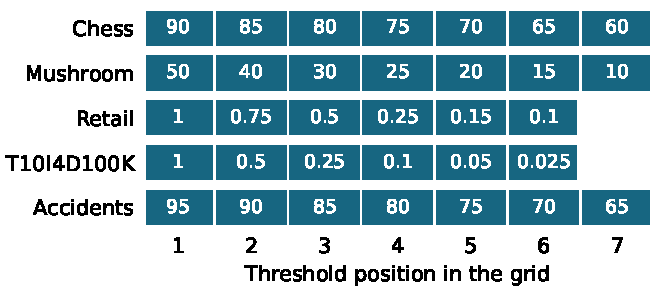
\includegraphics[width=\columnwidth]{figures/en/correctness-grid.pdf}
\caption{Minsup grid per database. Each cell gives minsup as a percentage and marks a
point where both variants match SPMF on every itemset and support.}
\label{fig:exact-grid}
\end{figure}

\begin{table}[t]
\centering
\caption{Thresholds whose full output matches SPMF, and the number of reference itemsets}
\label{tab:bench-exact}
\begin{tabular}{lrrr}
\hline
Data & Baseline & Optimized & Itemset range \\
\hline
Chess & 7/7 & 7/7 & 622--254\,944 \\
Mushroom & 7/7 & 7/7 & 153--574\,431 \\
Retail & 6/6 & 6/6 & 159--7\,589 \\
T10I4D100K & 6/6 & 6/6 & 385--96\,959 \\
Accidents & 7/7 & 7/7 & 15--1\,093 \\
\hline
\end{tabular}
\end{table}

\subsubsection{Process peak memory}
The same campaign records the peak RSS of every run. The measurement covers start-up,
reading the data, mining, and writing the whole output. Table~\ref{tab:peak-rss} gives
the medians at the lowest minsup of each database, where the output and the search are
largest. Every program reports at least 252\,MiB at every point, a floor set by the
measurement itself, so a value at that floor is only an upper bound.

\begin{table}[t]
\centering
\small
\setlength{\tabcolsep}{3pt}
\caption{Median peak RSS (MiB) over five repeats at the lowest minsup of each database.
$R$ is the baseline's median divided by the optimized variant's.}
\label{tab:peak-rss}
\begin{tabular}{lrrrrr}
\hline
Data / minsup & Baseline & Optimized & $R$ & SPMF & PrePost+ \\
\hline
Chess / 0.6 & 285.1 & 261.5 & 1.090 & 526.5 & $\le 254$ \\
Mushroom / 0.1 & 366.0 & 299.2 & 1.223 & 514.2 & $\le 254$ \\
Retail / 0.001 & 289.6 & 280.9 & 1.031 & 844.4 & $\le 254$ \\
T10I4D100K / 0.00025 & 303.7 & 278.5 & 1.090 & 556.0 & 297.4 \\
Accidents / 0.65 & 608.4 & 398.3 & 1.528 & 4\,248.1 & 340.9 \\
\hline
\end{tabular}
\end{table}

From the medians in the table, the percentage reduction is $100(1-M_o/M_b)$, where $M_b$
and $M_o$ are the median peak RSS of the baseline and the optimized variant. The reduction
ranges from 3.0\% on Retail to 34.5\% on Accidents. SPMF Eclat uses 1.7 to 10.7 times as
much as the optimized variant. PrePost+ uses less on Accidents (340.9 against
398.3\,MiB) and stays at the floor on Chess, Mushroom, and Retail. The optimized variant uses \emph{bitsets} (bit
arrays) and reuses buffers when it intersects tidsets in Eclat's prefix
search~\cite{zaki2000}. For a database of $N$ transactions, a tidset with $s$ tids takes
$8s$ bytes as a list of 64-bit integers and $8\lceil N/64\rceil$ bytes as a bit array,
counting elements only. The bit array saves space for long tidsets, and the optimized
variant can switch classes with short tidsets to lists. Peak RSS combines the data, the
search structures, the result, and the runtime's own memory. The numbers show the
whole-process difference at the chosen thresholds.

\subsection{Runtime, output size, and scalability}
\subsubsection{Runtime against minimum support}
\label{sec:minsup}
We timed four programs in a single session on the grading machine
(Section~\ref{sec:protocol}): the baseline, the optimized variant, SPMF 2.66 Eclat, and
SPMF PrePost+. Both Julia variants ran through the \texttt{demo.jl} command-line
interface at the same revision (\texttt{ca60f43}), so the times use the \emph{process}
scope: from process launch until the output file is written, including Julia or JVM
start-up, reading, and writing. The grid has 33 (benchmark, minsup) points on the five
benchmarks of Table~\ref{tab:datasets}, and each point was repeated five times. All 660
runs were checked itemset by itemset against an independent SPMF Eclat run and matched
exactly.

Each point is the median of its five repeats. The interquartile range relative to the
median is at most 2.9\% for the baseline and 1.9\% for the optimized variant at every
point. For SPMF and PrePost+ it reaches 11.3\% and 13.9\%, and only one SPMF point and
three PrePost+ points exceed 10\%. To estimate drift between sessions, we compared with
three other sessions on the same machine. The PrePost+ times (the same Java command) of
this session differ by $+3.0\%$, $+1.9\%$, and $-2.3\%$ in geometric mean, and by at most
14.4\% at a single point. The optimized variant measured in another session at the same
revision differs by $-1.5\%$ on average and at most 5.6\%. The four programs in the tables
ran in the same session, so a ratio between two of them carries only within-session
noise. We treat a ratio as a real difference when it exceeds the sum of the two largest
interquartile ranges: about 5\% between the two Julia variants and about 16\% when one
side is a Java program. Drift between sessions matters only when comparing with another
campaign, at 5.6\% for the optimized variant and 14.4\% for PrePost+.

\begin{figure*}[t]
\centering
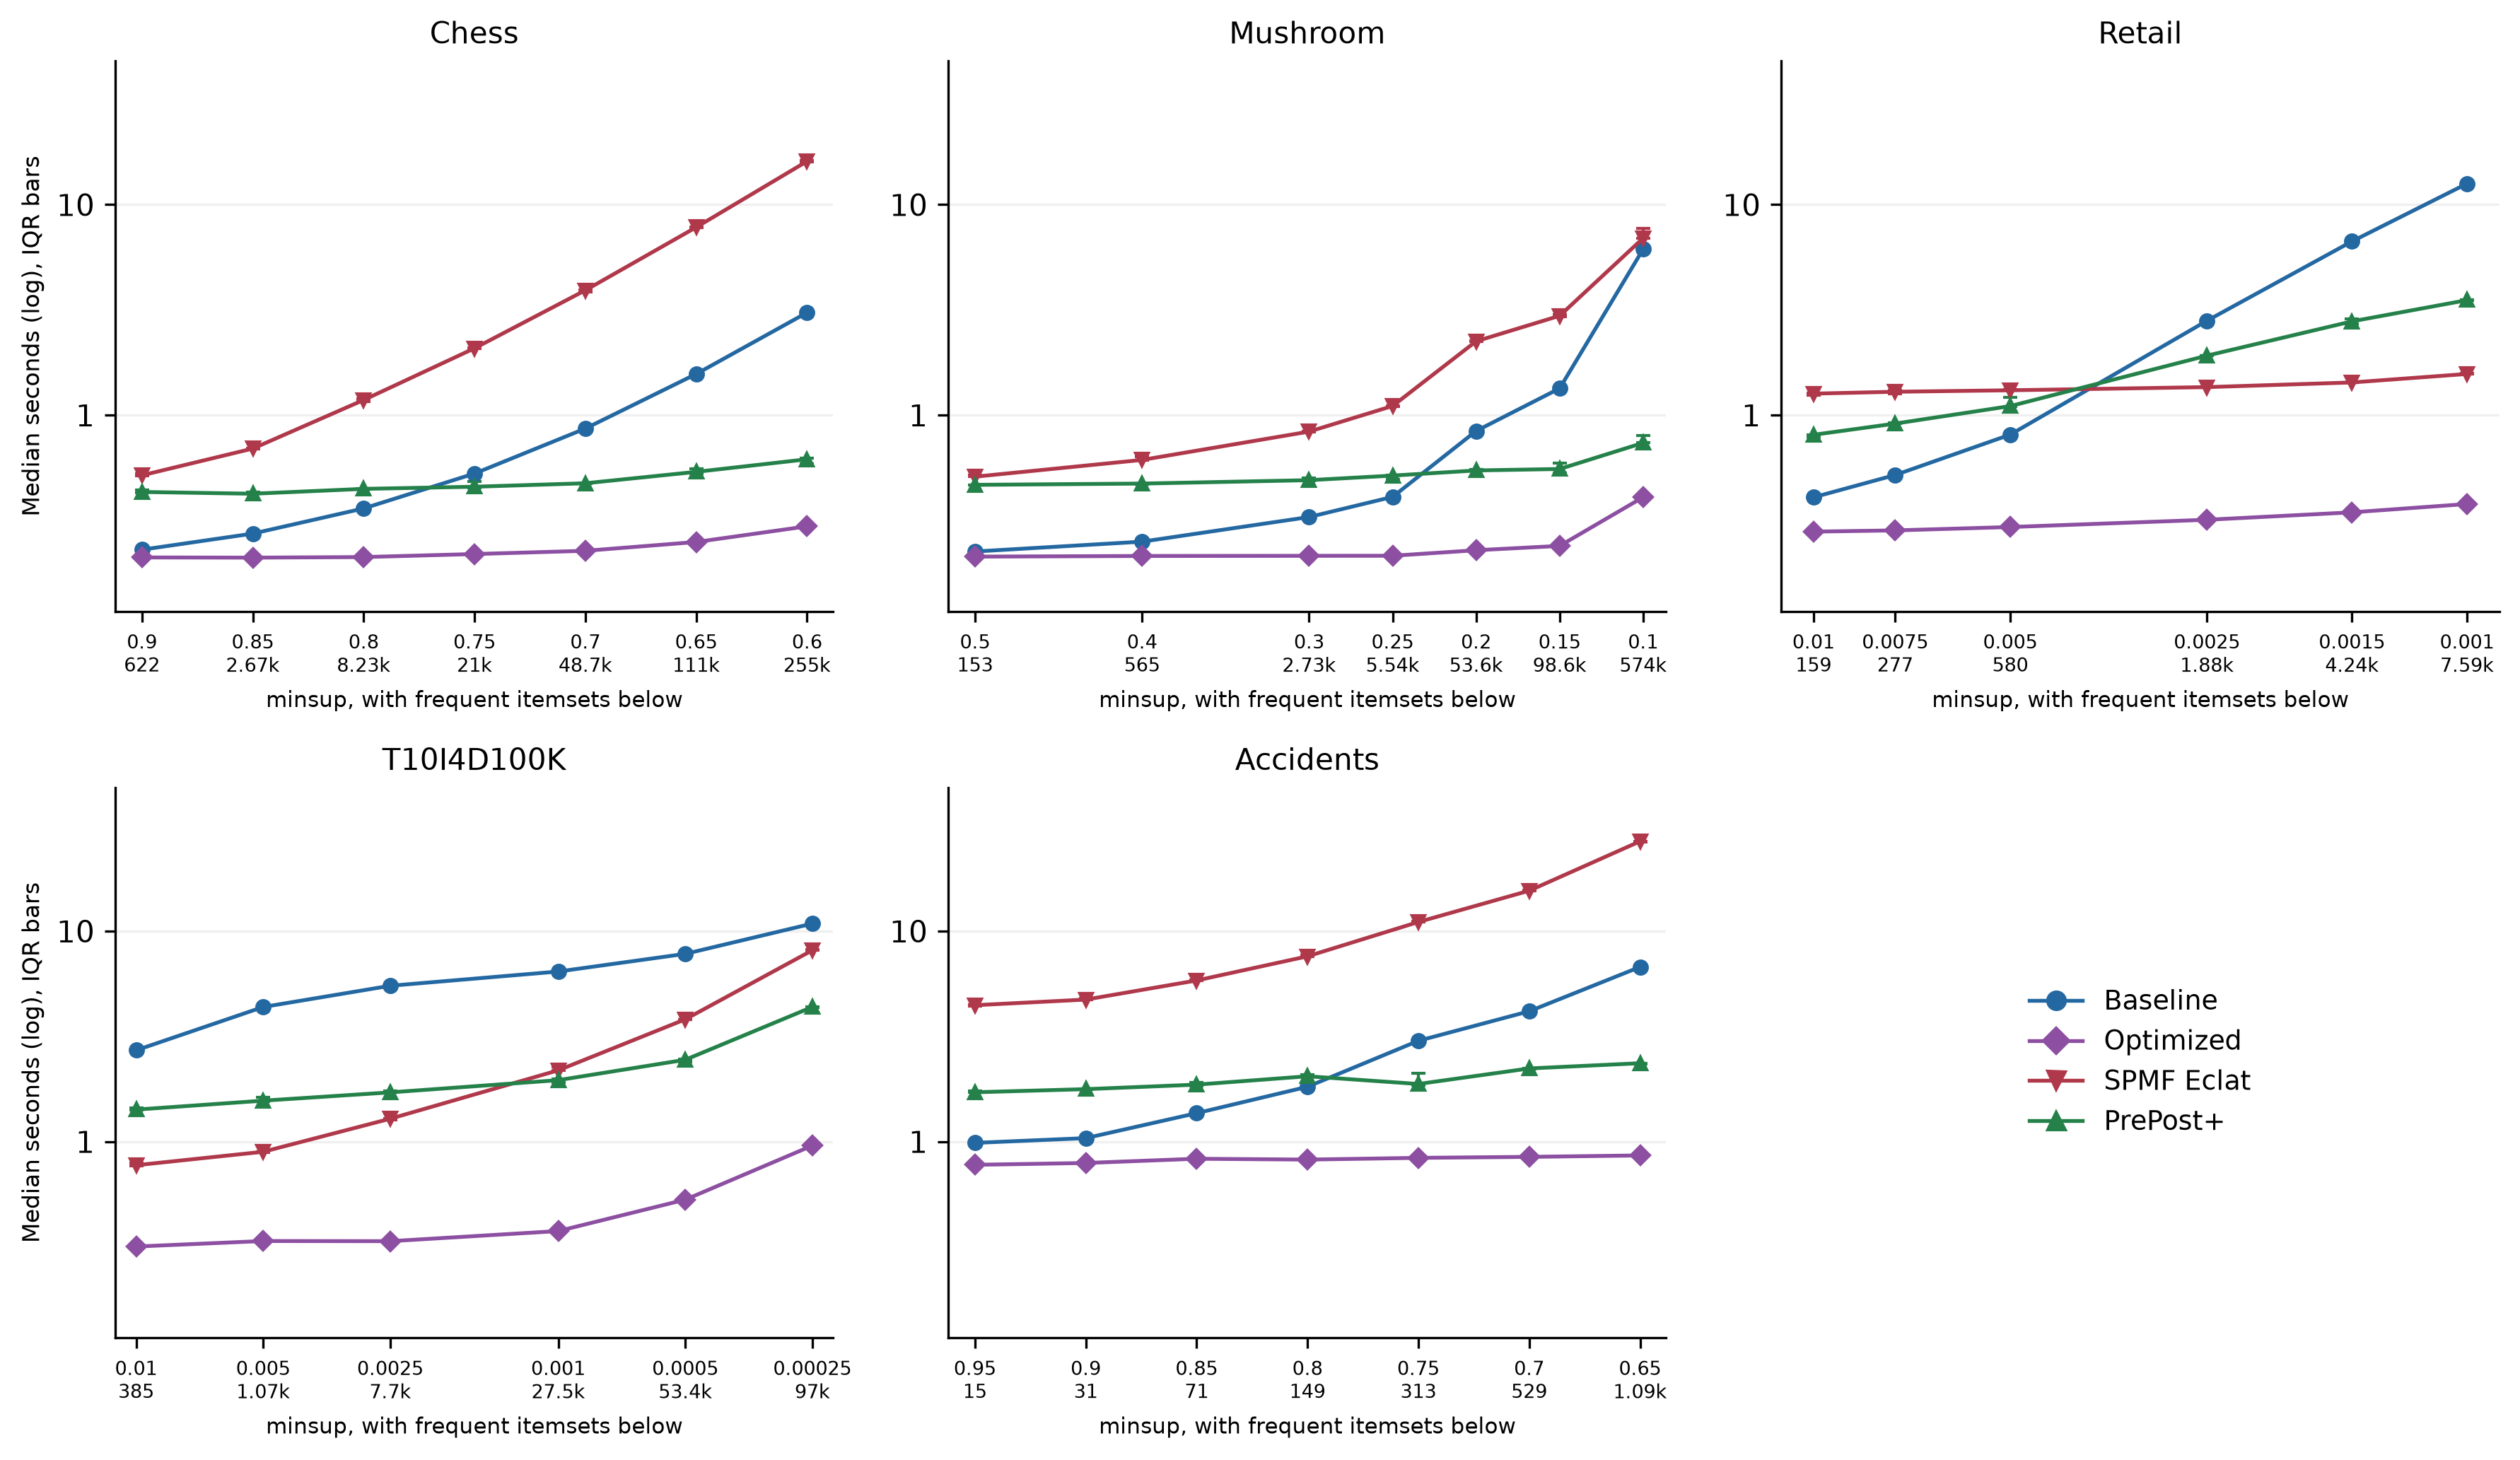
\includegraphics[width=\textwidth]{figures/runtime-curves.png}
\caption{\emph{Process} time against minsup for the four programs on the five
benchmarks. The vertical axis is logarithmic, points are medians of five repeats, and bars
are interquartile ranges. Below each horizontal-axis label is the number of frequent
itemsets.}
\label{fig:runtime}
\end{figure*}

The optimized variant is the fastest at all 33 points, at 0.21 to 0.96\,s. At the lowest
minsup of each benchmark (Table~\ref{tab:runtime-low}) it is faster than the baseline by
about 7.9 times on Accidents, 10.4 on Chess, 11.3 on T10I4D100K, 15.1 on Mushroom, and
33.3 on Retail. Table~\ref{tab:runtime-ratio} gives the geometric mean of this ratio over
every point of each benchmark, together with the ratios of SPMF Eclat and PrePost+ to the
optimized variant.

\begin{table}[t]
\centering
\footnotesize
\setlength{\tabcolsep}{3pt}
\caption{\emph{Process} time (seconds) at the lowest minsup of each benchmark, median of
five repeats. ``Sets'' is the number of frequent itemsets.}
\label{tab:runtime-low}
\begin{tabular}{lrrrrrr}
\hline
Data / minsup & Sets & Baseline & Optimized & SPMF & PrePost+ \\
\hline
Chess / 0.6 & 254\,944 & 3.07 & 0.30 & 16.07 & 0.62 \\
Mushroom / 0.1 & 574\,431 & 6.15 & 0.41 & 6.93 & 0.74 \\
Retail / 0.001 & 7\,589 & 12.59 & 0.38 & 1.57 & 3.52 \\
T10I4D100K / 0.00025 & 96\,959 & 10.86 & 0.96 & 8.11 & 4.36 \\
Accidents / 0.65 & 1\,093 & 6.76 & 0.86 & 26.70 & 2.36 \\
\hline
\end{tabular}
\end{table}

\begin{table}[t]
\centering
\small
\setlength{\tabcolsep}{4pt}
\caption{Geometric mean over every point of each benchmark of the \emph{process} time
ratio: the time of the program named in the column header divided by the time of the
optimized variant. A value above 1 means slower than the optimized variant.}
\label{tab:runtime-ratio}
\begin{tabular}{lrrr}
\hline
Data & Baseline & SPMF & PrePost+ \\
\hline
Chess & 2.83 & 10.33 & 2.08 \\
Mushroom & 2.73 & 6.01 & 2.22 \\
Retail & 5.89 & 4.34 & 5.01 \\
T10I4D100K & 13.14 & 4.53 & 4.76 \\
Accidents & 2.62 & 10.76 & 2.39 \\
\hline
\end{tabular}
\end{table}

The amount of work explains the shape of the baseline's curves. The baseline intersects
two sorted tidsets by merging them, so each intersection costs work proportional to the
combined length of the two tidsets. We reran the baseline's search on one thread and
counted the intersections (joins), the intersections that produced a frequent itemset,
and the combined length of the two tidsets over all intersections, which we call merged
elements (Table~\ref{tab:join-work}). Subtracting the time at the highest minsup (mostly
start-up and file reading) from the time at the lowest minsup and dividing by the
difference in merged elements, the baseline spends 2.0 to 6.9\,ns per element across the
five benchmarks. That is the same order as the 9.0 to 10.0\,ns from the transaction-length
experiment in Section~\ref{sec:width}.

\begin{table}[t]
\centering
\small
\setlength{\tabcolsep}{3pt}
\caption{Work done by the baseline at the lowest minsup of each benchmark. ``Success'' is
the share of intersections that produce a frequent itemset, ``Elements'' is the combined
length of the two tidsets over all intersections (billions), and ns/el is the time per
merged element after subtracting the time at the highest minsup.}
\label{tab:join-work}
\begin{tabular}{lrrrr}
\hline
Data / minsup & Joins & Success & Elements & ns/el \\
\hline
Chess / 0.6 & 326\,545 & 78.1\% & 1.43 & 2.0 \\
Mushroom / 0.1 & 722\,721 & 79.5\% & 1.66 & 3.6 \\
Retail / 0.001 & 3\,932\,582 & 0.14\% & 2.17 & 5.7 \\
T10I4D100K / 0.00025 & 4\,192\,075 & 2.3\% & 1.48 & 6.9 \\
Accidents / 0.65 & 2\,333 & 46.1\% & 1.22 & 4.8 \\
\hline
\end{tabular}
\end{table}

The structure of the data decides that work. On Chess and Mushroom, the number of
intersections is only 1.26 to 1.28 times the number of frequent itemsets and about 78\%
to 80\% of intersections succeed, so work grows with the number of frequent itemsets. On
Retail, minsup 0.001 produces 3.93 million intersections but only 5\,472 succeed, so each
frequent itemset costs about 286\,000 merged elements, and the baseline takes 12.59\,s,
8.0 times SPMF Eclat (1.57\,s) and 3.6 times PrePost+ (3.52\,s) at the same point. On
T10I4D100K, even minsup 0.01 needs 70\,127 intersections and 297.7 million merged
elements to produce exactly 10 two-item sets, so the baseline-to-optimized ratio is
already 8.5 at the first point. The optimized variant's curve is nearly flat and rises
clearly only at the points with the largest output (Mushroom 0.1, T10I4D100K 0.00025).
Section~\ref{sec:future} analyzes where the optimized variant spends its time.

At the highest minsup of Chess, Mushroom, Accidents, and Retail, the baseline-to-optimized
ratio is only 1.09, 1.06, 1.27, and 1.46. All four exceed the within-session noise
between the two Julia variants (about 5\%), so they are real differences, but small ones.
On Chess and Mushroom the gap is a few percent of a run that is mostly start-up and file
reading. On Accidents and Retail the absolute gap is only 0.21\,s and 0.13\,s, the same
order as start-up and file reading (about 0.21\,s on Chess at minsup 0.9, a point that
consists almost entirely of those steps). These ratios therefore do not show that the two
algorithms are equally fast. At the lowest minsup, SPMF Eclat is faster than the
baseline on Retail (8.0 times) and T10I4D100K (1.3 times) but slower on Chess (5.2 times)
and Accidents (4.0 times). On Mushroom, SPMF Eclat takes 6.93\,s and the baseline
6.15\,s. The 13\% gap is within the noise of a Java program (about 16\%), so the two
programs cannot be told apart. We treat SPMF as a black box, so we do not explain the
reversal at the other points.

These conclusions have limits: one machine, five repeats per point, and a
\emph{process} scope that includes Julia or JVM start-up (the Java programs also pay for
JVM start-up). The baseline is the version at revision \texttt{ca60f43}, which already
benefits from the faster reading and writing of later stages, so it is not the baseline
measured on 2026-10-31. The intersection counts come from a separate run, outside the
timed runs.

\subsubsection{Number of frequent itemsets against minsup}
\label{sec:output-size}
The output sizes come from the timing campaign of 2026-11-17 on 33 thresholds of the
five databases, shown in Fig.~\ref{fig:output-size}, so no extra mining was needed. That
campaign ran the baseline, the optimized variant, SPMF's Eclat, and PrePost+ five times
each at every threshold, and all 660 outputs match SPMF's Eclat exactly. The script
\texttt{scripts/output\_size.jl} checks three more properties on the kept outputs. First,
the four programs report the same number of itemsets at every threshold. Second, the
count never falls as minsup falls: by the anti-monotone property, every subset of a
frequent itemset is frequent, so lowering the threshold cannot lose an itemset. Third,
the outputs are nested: for each pair of adjacent thresholds $\sigma_1 > \sigma_2$, the
itemsets with support at least $\sigma_1$ in the output at $\sigma_2$ are exactly the
output at $\sigma_1$, with the same supports. Support does not depend on the threshold, so
this check catches a support that is wrong in only one run. All 28 threshold pairs
satisfy all three properties.

\begin{figure*}[t]
\centering
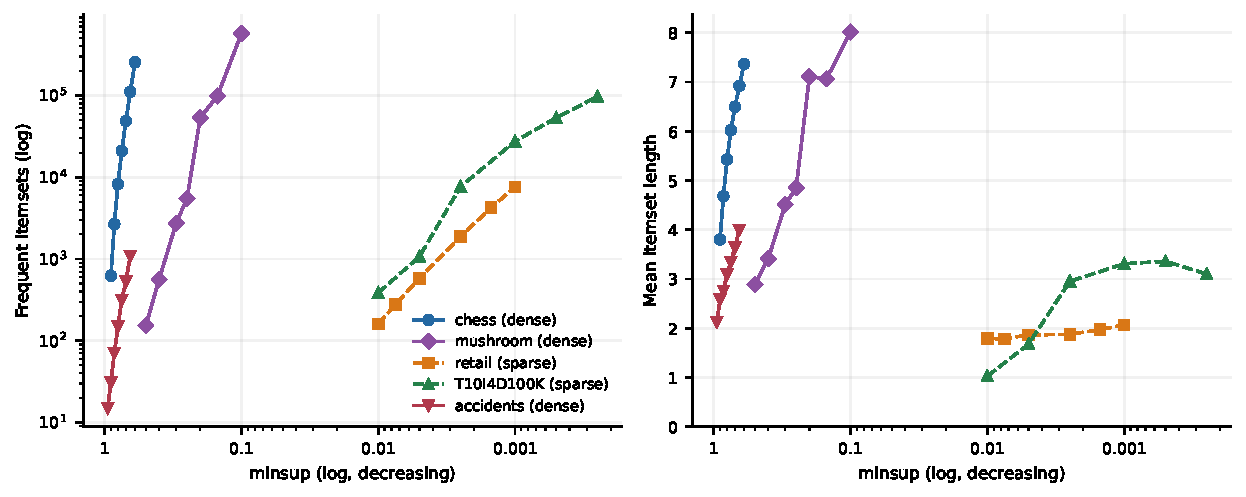
\includegraphics[width=\textwidth]{figures/en/output-size.pdf}
\caption{Number of frequent itemsets (left, log scale) and mean frequent-itemset length
(right) as minsup decreases on the five databases. Solid lines are dense data and dashed
lines are sparse data.}
\label{fig:output-size}
\end{figure*}

Fig.~\ref{fig:output-size} shows that the number of frequent itemsets grows much faster
on dense data. To compare growth rates across databases with different minsup ranges, we
fit the model
\begin{equation}
  \log F = c - s \log(\mathrm{minsup}),
  \label{eq:output-growth}
\end{equation}
where $F$ is the number of frequent itemsets at a threshold, $c$ is a per-database
constant, and $s$ is the slope on a log-log scale: when minsup falls by a factor $q$, $F$
grows by about $q^s$. Table~\ref{tab:output-growth} shows $s$ from 5.2 to 14.3 on the
three dense databases, but only 1.6 and 1.7 on the two sparse ones. Chess grows 410-fold
when minsup only drops from 0.9 to 0.6, while Retail grows 48-fold when minsup drops
tenfold.

\begin{table}[t]
\centering
\small
\caption{Number of frequent itemsets $F$ at the highest and lowest threshold, slope $s$
of model~\eqref{eq:output-growth}, and maximum frequent-itemset length $k_{\max}$ at the
lowest threshold}
\label{tab:output-growth}
\setlength{\tabcolsep}{4pt}
\begin{tabular}{lrrrrr}
\hline
Data & minsup & $F$ high & $F$ low & $s$ & $k_{\max}$ \\
\hline
Chess & 0.9--0.6 & 622 & 254\,944 & 14.3 & 14 \\
Accidents & 0.95--0.65 & 15 & 1\,093 & 11.3 & 8 \\
Mushroom & 0.5--0.1 & 153 & 574\,431 & 5.2 & 16 \\
Retail & 0.01--0.001 & 159 & 7\,589 & 1.7 & 5 \\
T10I4D100K & 0.01--0.00025 & 385 & 96\,959 & 1.6 & 11 \\
\hline
\end{tabular}
\end{table}

Itemset length explains the difference. In dense data, each transaction contains a large
share of the items, so many items occur together in most transactions and form long
frequent itemsets. A frequent $k$-itemset brings $2^k - 1$ non-empty subsets that are also
frequent, so whenever a lower threshold admits longer itemsets, the count grows
exponentially in their length. Mean length on Chess rises from 3.8 to 7.4 and on
Mushroom from 2.9 to 8.0 across the threshold grid. Mushroom grows 9.7-fold, from 5\,545
to 53\,583 itemsets, when minsup drops from 0.25 to 0.2, and at that same step the
maximum length rises from 11 to 15. In sparse data, transactions are short and items
rarely occur together, so lowering the threshold mostly adds single items and pairs. Mean
length on Retail stays between 1.8 and 2.1. On T10I4D100K 0.00025, 45\,660 of the 96\,959
itemsets, or 47\%, are 2-itemsets.

The number of frequent itemsets does not decide runtime on its own. In the same campaign,
the baseline takes 12.59 s on Retail 0.001 with 7\,589 itemsets, but only 3.07 s on
Chess 0.6 with 254\,944 itemsets. By~\eqref{eq:cost}, the cost is the number of
intersections times tidset length, not the number of results. Retail has 2\,117 frequent
items, so the root class has over two million pairs to intersect, and most of those
intersections fail without producing any itemset (Section~\ref{sec:optimized}). The
optimized variant avoids most of these intersections by counting pairs and runs Retail
0.001 in 0.38 s. Even with the optimized variant, Mushroom 0.1 with 574\,431 itemsets
takes 0.41 s, while T10I4D100K 0.00025 with 96\,959 itemsets takes 0.96 s, because
T10I4D100K's tidsets span 100\,000 transactions and most intersections at depth 2 fail.
The count dominates runtime only when it is very large: on Mushroom 0.05, before radix
sort, sorting and writing 3\,755\,511 itemsets took 89\% of the time and mining only 11\%
(Section~\ref{sec:optimized}). Conversely, when relative minsup is fixed, the count barely
changes, and runtime grows with $N$, as Section~\ref{sec:scalability} shows.

\subsubsection{Effect of transaction length}
\label{sec:width}
To separate transaction length from the density and output volume that are mixed together
in real benchmarks, we generated eight synthetic databases with the same $N = 10\,000$
transactions and $|I| = 100$ items, differing only in transaction length
$w \in \{5, 10, \dots, 40\}$. In the sampling model, each transaction is a uniformly random
subset of exactly $w$ items, independent of the other transactions, so the items are
interchangeable and no pair occurs together more often than chance. A $k$-itemset
therefore has expected support $N \prod_{j=0}^{k-1} (w - j)/(|I| - j)$; for example, a
pair appears in $N\,w(w-1)/(|I|(|I|-1))$ transactions. The generator uses SplitMix64 with
seed $(42 \ll 32) \,|\, w$ instead of Julia's \texttt{Xoshiro}, because Julia does not
guarantee the same random stream across versions. This keeps the SHA-256 hashes in the
manifest valid on every platform.

Two confounding factors need separating. The first is output volume: longer transactions
push more pairs and triples over the threshold, so the number of frequent itemsets grows
in steps, and runtime follows that count rather than necessarily following $w$. The second
is co-occurrence. The model removes it by keeping items independent, so the results
cannot stand in for the behavior of Chess or Mushroom. We therefore measure under two
protocols. The fixed protocol uses $\mathrm{minsup} = 0.05$ at every $w$. The
matched-output protocol uses, for each $w$, the largest threshold $\sigma$ that still
gives at least 5\,000 frequent itemsets, so output stays nearly constant and $w$ is the
only thing that changes.

Under the fixed protocol, the number of frequent itemsets is 53, 100, 100, 100, 5\,050,
5\,050, 5\,050, and 166\,749 as $w$ grows from 5 to 40. Pairs start to reach
$\sigma = 500$ at $w = 25$ (expected support 606, against 384 at $w = 20$), and triples at
$w = 40$ (expected 611). The baseline Eclat's runtime follows these steps (1.0\,s at
$w = 20$, 2.9\,s at $w = 25$, 49.4\,s at $w = 40$ in the \emph{process} scope,
Fig.~\ref{fig:width}), so a plot against $w$ at one minsup mostly reflects output, not
transaction length.

\begin{figure*}[t]
\centering
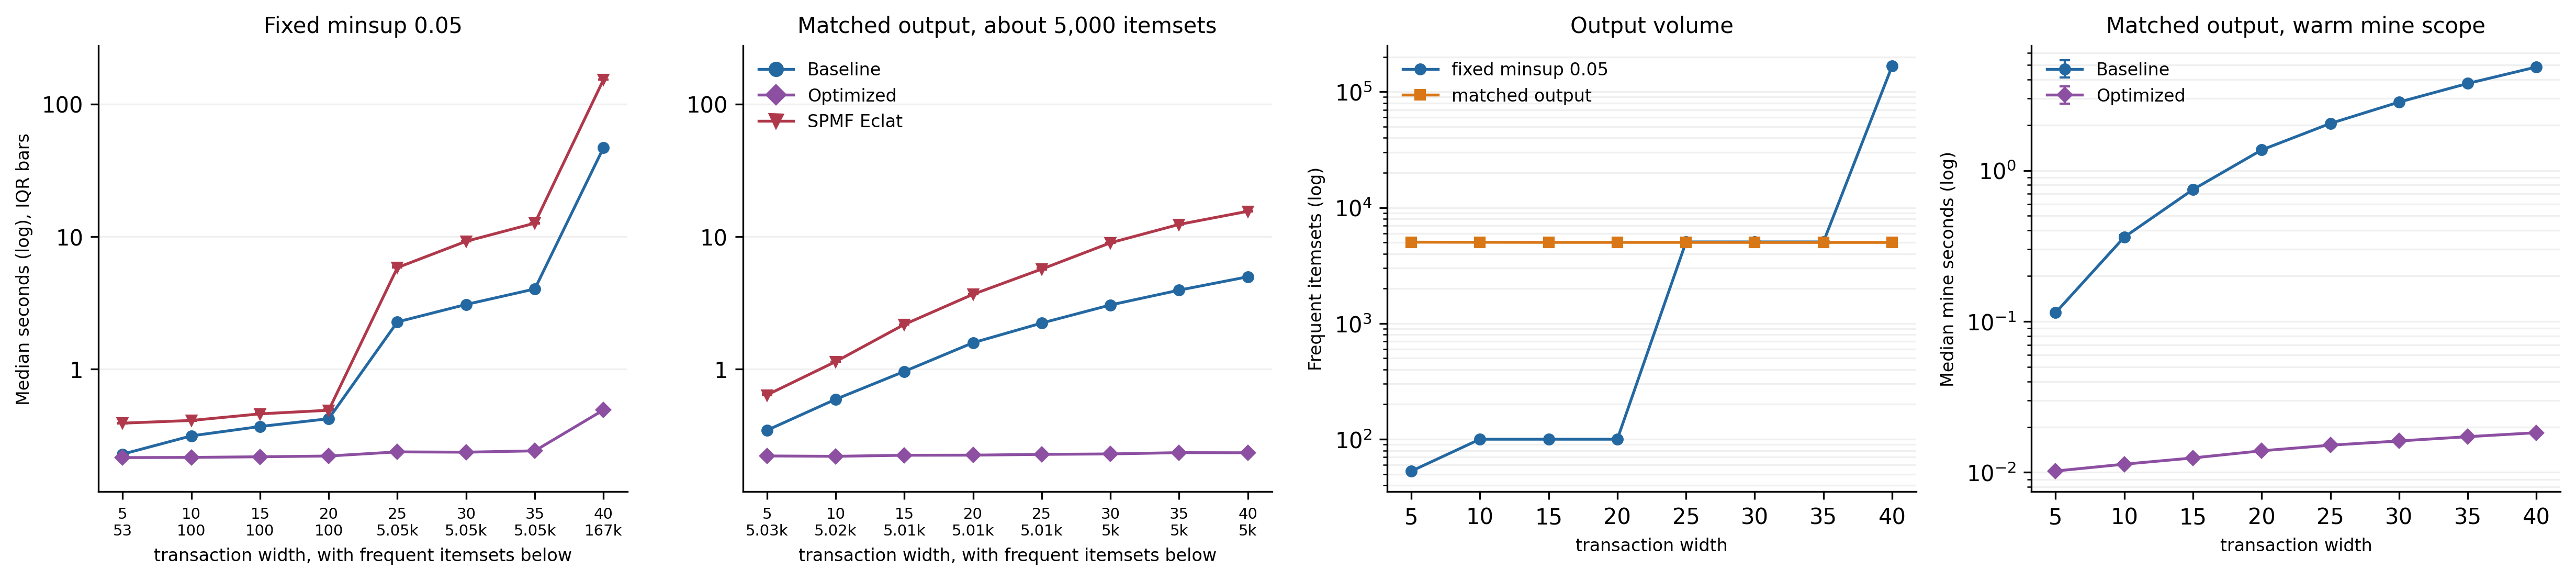
\includegraphics[width=\textwidth]{figures/width-curves.png}
\caption{Runtime and output volume against transaction length $w$ on the synthetic
databases ($N = 10\,000$, $|I| = 100$). From left to right: \emph{process} time at fixed
minsup 0.05; \emph{process} time with output matched to about 5\,000 itemsets; number of
frequent itemsets under both protocols; \emph{mine} time (after warm-up) with matched
output. Medians of three repeats with interquartile-range bars; below each axis label is
the number of frequent itemsets.}
\label{fig:width}
\end{figure*}

Under the matched-output protocol, the number of frequent itemsets stays around 5\,000 and
the number of tidset intersections (joins) is nearly constant (about 164\,000, of which
about 4\,900 succeed), but the baseline Eclat's mining time grows 42-fold as $w$ goes from
5 to 40 (Table~\ref{tab:width}). The reason is that the baseline intersects two sorted
tidsets by merging them, so each intersection costs work proportional to their combined
length. Each item appears in a fraction $w/|I|$ of the transactions, so its tidset length
is proportional to $w$, and the tidset of a pair is proportional to $w(w-1)$. The total
number of merged elements grows 47-fold while $w$ grows only 8-fold, and the baseline's
time tracks it at 9.0 to 10.0\,ns per element. The optimized variant intersects bitsets of
$\lceil N/64 \rceil = 157$ machine words regardless of tidset length, so its mining time
grows only 1.8-fold, from 10.2 to 18.3\,ms. In the \emph{process} scope, the optimized
variant is nearly flat at 0.79 to 0.80\,s because Julia start-up and compilation dominate.
We have not identified the source of that 1.8-fold growth. Under both protocols every
output matches SPMF exactly.

\begin{table}[t]
\centering
\caption{Eclat under the matched-output protocol. $\sigma$ is the threshold in
transactions, ``Elements'' is the combined length of the two tidsets over all of the
baseline's intersections, and times are \emph{mine} medians of three repeats.}
\label{tab:width}
\begin{tabular}{rrrrrr}
\hline
$w$ & $\sigma$ & Sets & Elements (M) & Baseline (s) & Optimized (ms) \\
\hline
5 & 10 & 5\,028 & 11.4 & 0.114 & 10.2 \\
10 & 69 & 5\,016 & 38.9 & 0.361 & 11.3 \\
15 & 179 & 5\,007 & 82.4 & 0.747 & 12.5 \\
20 & 340 & 5\,007 & 142.0 & 1.366 & 13.9 \\
25 & 550 & 5\,007 & 217.2 & 2.046 & 15.1 \\
30 & 815 & 5\,002 & 308.8 & 2.833 & 16.2 \\
35 & 1\,127 & 5\,002 & 416.4 & 3.765 & 17.2 \\
40 & 1\,488 & 5\,001 & 538.8 & 4.841 & 18.3 \\
\hline
\end{tabular}
\end{table}

As for the search tree, with minsup fixed the tree both deepens by one level at $w = 25$
(pairs) and $w = 40$ (triples) and widens: the number of intersections grows from 4\,950
to 166\,650 and then 4\,087\,798. With output matched, the tree has the same size at every
$w$, so only the cost per intersection changes. The scope of these conclusions is
limited: one $N$ and one item count, eight values of $w$, independent items, three
repeats on one machine, and a target of 5\,000 itemsets that is a choice, not a
derived value.

\subsubsection{Scalability}
\label{sec:scalability}
This experiment asks whether runtime grows linearly or nonlinearly with the number of
transactions $N$ when the database grows and the relative threshold stays fixed. We chose
Accidents, the largest database in Table~\ref{tab:datasets}, and Retail, the sparse
database with the most items. Each database was shuffled once with seed 42, and the $p\%$
subset holds the first $p\%$ of transactions of that permutation, with
$p \in \{10, 25, 50, 75, 100\}$. The subsets are therefore nested: a larger subset only
adds transactions and never replaces those of a smaller one, so the difference between two
points comes only from the added data. The script \texttt{experiments/prepare\_subsets.jl}
regenerates the subsets, and the SHA-256 hash of each file is recorded in
\texttt{data/benchmark/subsets.toml}. Mean transaction length barely changes between
subsets, from 33.79 to 33.81 on Accidents and from 10.30 to 10.37 on Retail, so sampling
does not change the shape of the data.

The threshold stays at minsup 0.65 for Accidents and 0.001 for Retail, the lowest
thresholds of each database in the runtime grid. The absolute threshold therefore grows
with $N$, from $\sigma = 22\,112$ to $221\,119$ on Accidents and from 9 to 89 on Retail.
The four programs were timed through the command line, each run in a fresh process, with
five interleaved repeats.
All 200 outputs match an independent SPMF Eclat run exactly. The interquartile range stays
within 1.9\% of the median for our two variants and 7.6\% for the two SPMF programs.

\begin{figure*}[t]
\centering
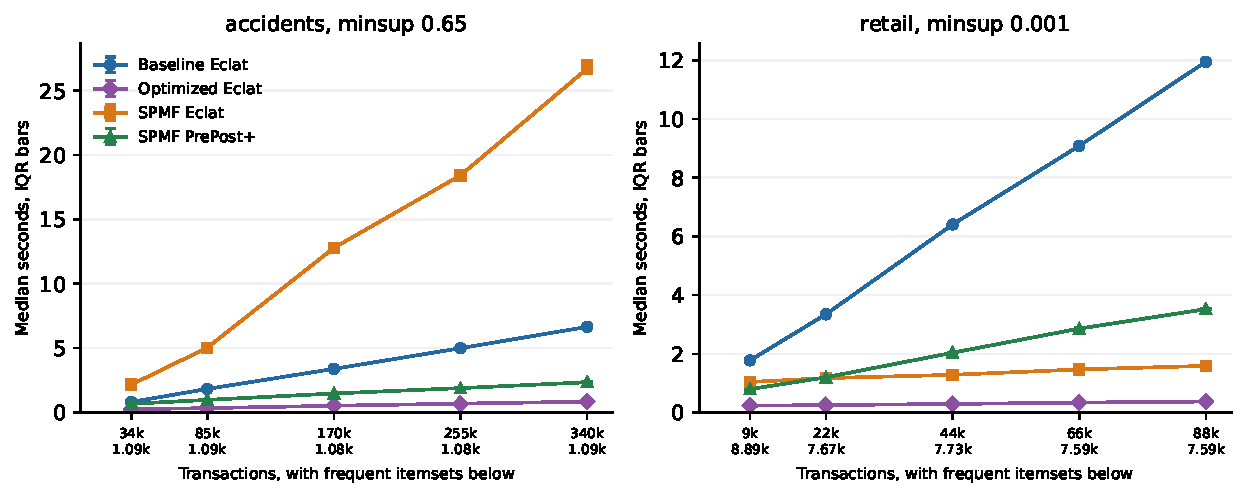
\includegraphics[width=\textwidth]{figures/en/scalability.pdf}
\caption{Median process time against number of transactions on five nested subsets of
Accidents (minsup 0.65) and Retail (minsup 0.001); error bars are the interquartile range
of five runs. The second row of numbers under the horizontal axis is the number of
frequent itemsets in each subset.}
\label{fig:scalability}
\end{figure*}

Fig.~\ref{fig:scalability} shows that all eight lines are close to straight. To check,
we fit each line with the model
\begin{equation}
  T(N) = a + b\,N,
  \label{eq:linear-fit}
\end{equation}
where $T(N)$ is the median time (seconds) on the subset with $N$ transactions, $a$ is a
fixed cost that does not depend on the data, and $b$ is the marginal cost per transaction.
The coefficient of determination $R^2$ is the share of the variance of $T$ that the model
explains, equal to 1 when the five points lie exactly on a line.
Table~\ref{tab:scalability-fit} shows $R^2 \ge 0.992$ for every line, so within the
measured range the runtime of all four programs grows linearly with $N$.

\begin{table}[t]
\centering
\small
\caption{Coefficients of model~\eqref{eq:linear-fit}: fixed cost $a$ (s), marginal cost
$b$ (s per 100\,000 transactions), coefficient of determination $R^2$, and the time ratio
between the 100\% and 10\% subsets}
\label{tab:scalability-fit}
\setlength{\tabcolsep}{4pt}
\begin{tabular}{llrrrr}
\hline
Data & Program & $a$ & $b$ & $R^2$ & $T_{100}/T_{10}$ \\
\hline
Accidents & Baseline & 0.19 & 1.90 & 0.9999 & 8.1 \\
 & Optimized & 0.19 & 0.20 & 0.9986 & 3.3 \\
 & SPMF Eclat & $-1.16$ & 8.02 & 0.9951 & 12.3 \\
 & PrePost+ & 0.52 & 0.54 & 0.9987 & 3.5 \\
Retail & Baseline & 0.61 & 12.87 & 0.9996 & 6.7 \\
 & Optimized & 0.22 & 0.18 & 0.9978 & 1.6 \\
 & SPMF Eclat & 1.00 & 0.69 & 0.9923 & 1.5 \\
 & PrePost+ & 0.48 & 3.51 & 0.9983 & 4.4 \\
\hline
\end{tabular}
\end{table}

The complexity analysis~\eqref{eq:cost} explains this trend. When relative minsup is
fixed, the set of frequent itemsets barely changes: Accidents has 1\,079 to 1\,095 frequent
itemsets at all five sizes. The equivalence classes visited are therefore the same, so the
number of intersections $C$ is nearly constant. Meanwhile the total length $L$ grows in
proportion to $N$, and each intersection costs time proportional to tidset length, which
is also roughly proportional to $N$, because a random sample keeps the share of
transactions that contain each itemset nearly the same. With bitsets, an intersection
reads $\lceil N/64 \rceil$ machine words, so the conclusion holds. All three terms are
linear in $N$, and no step of Eclat depends on the square of the number of transactions.

The fixed cost $a$ of the optimized variant is 0.19 s on Accidents and 0.22 s on Retail,
close to the Julia start-up and package-loading time of Section~\ref{sec:measure}. Because
this fixed part dominates on the small subsets, the optimized variant's time grows only
3.3-fold on Accidents and 1.6-fold on Retail when $N$ grows tenfold, even though the line
is straight. The coefficient $b$ is the quantity to compare for scalability: the
baseline's marginal cost is 9.7 times the optimized variant's on Accidents and 71 times on
Retail. On Retail, the baseline intersects every pair of frequent items at the root on tid
lists whose length is proportional to $N$, while the optimized variant counts pairs in one
pass over the horizontal database and intersects only the pairs that reach the threshold.
The time ratio between the two variants therefore grows from 7.7 on the 10\% subset to
31.9 on the 100\% subset. The optimized variant is faster than PrePost+ at all ten points,
with $R$ from 0.35 to 0.38 on Accidents and from 0.29 down to 0.11 on Retail, because the
marginal cost of PrePost+ is 2.8 times larger on Accidents and 19 times larger on Retail.

Two factors other than $N$ could change the amount of work between subsets, and we
measured both. The first is the number of distinct items, which grows with $N$ from 343 to
468 on Accidents and from 10\,208 to 16\,470 on Retail. The number of frequent items barely
changes: exactly 18 items in all five Accidents subsets, and 2\,100 to 2\,270 on Retail, so
the new items are all rare and drop out in the first counting pass. The second is that on
Retail 10\%, the absolute threshold is only $\sigma = 9$. In a small sample, the support of
itemsets whose true support sits just below the threshold fluctuates more, and because
there are very many such itemsets, more of them rise above the threshold than fall below
it. The 10\% subset therefore has 2\,270 frequent items, the most of the five subsets, and
8\,895 frequent itemsets, 17\% more than the 7\,589 of the full database. This extra work
is small next to the growth with $N$: the point farthest from the fitted line is only
4 ms off for the optimized variant on Retail and 0.12 s off for the baseline, which is 1\%
of the time on the 100\% subset.

SPMF's Eclat is the only program with signs of nonlinearity. On Accidents its time grows
12.3-fold when $N$ grows tenfold, the quadratic term of the fit is positive, and its $R^2$
of 0.9951 is the lowest of the four Accidents rows. Because the curve bends upward, the
fitted line crosses the vertical axis at a negative value, so $a$ in that row is not a
fixed cost. We did not measure SPMF's internal structure, so we
only record this trend and do not attribute it to a specific cause.

\subsection{Analysis and future directions}
\label{sec:future}
The assignment suggests two optimization directions: an adaptive tidset representation
that switches between lists and \emph{bitsets}, and early termination of tidset
intersections. The optimized variant already has both: \texttt{prefer\_lists}
switches an equivalence class to lists when that is cheaper, \texttt{intersect\_lists!}
stops when the tids found so far plus the rest of the shorter list cannot reach minsup,
and \texttt{BlockCounts} rejects an intersection without merging. Diffsets were tried and
dropped because they were not faster than bitsets beyond noise. We therefore measured
where the optimized variant still spends its time before proposing anything.

\texttt{scripts/stage\_profile.jl} times the three stages of the CLI path (reading,
mining, and writing) in a warm process (median of five runs after one warm-up run). It
also samples with a \emph{profiler}, a tool that records which function is running, and
assigns each sample to the package function it was in. In
Table~\ref{tab:stage-profile}, ``Layout'' covers reading the file, counting items,
building the root bitsets, and checking the canonical form. ``Intersect'' covers bitset
and list intersections, converting bitsets to lists, block counting, and search
bookkeeping. ``Output'' covers node expansion, sorting, and formatting.

\begin{table}[t]
\centering
\footnotesize
\setlength{\tabcolsep}{1.5pt}
\caption{Share of \emph{profiler} samples by group, in percent, for the optimized
variant's CLI path. ``Run'' is the time of one read, mine, and write pass (seconds).
Chess 0.9 and Mushroom 0.5 take only 5 to 7\,ms, too short to sample.}
\label{tab:stage-profile}
\begin{tabular}{lrrrrrr}
\hline
Point & Itemsets & Run & Layout & Pairs & Intersect & Output \\
\hline
Chess 0.6 & 254\,944 & 0.099 & 5 & 0 & 12 & 83 \\
Mushroom 0.1 & 574\,431 & 0.180 & 4 & 0 & 1 & 95 \\
Mushroom 0.05 & 3\,755\,511 & 1.237 & 1 & 0 & 1 & 98 \\
Retail 0.01 & 159 & 0.069 & 98 & 0 & 1 & 0 \\
Retail 0.001 & 7\,589 & 0.144 & 57 & 39 & 4 & 1 \\
T10I4D100K 0.01 & 385 & 0.105 & 66 & 34 & 0 & 0 \\
T10I4D100K 0.00025 & 96\,959 & 0.710 & 10 & 7 & 79 & 5 \\
Accidents 0.95 & 15 & 0.567 & 98 & 0 & 0 & 2 \\
Accidents 0.65 & 1\,093 & 0.619 & 99 & 0 & 0 & 0 \\
\hline
\end{tabular}
\end{table}

Tidset intersection, the core operation of Eclat, takes most of the time at only one
point, T10I4D100K 0.00025. At the three dense points (Chess 0.6, Mushroom 0.1 and 0.05),
output takes 83\% to 98\%. At the other five points, building the vertical layout and
counting pairs dominate, and on Accidents the search takes under 1\% of the run. The
earlier subsections agree with this. On Accidents, the optimized variant's CLI time grows
linearly with the number of transactions even though the output barely changes (about
1\,100 itemsets), and its slope is the smallest of the four programs
(Table~\ref{tab:scalability-fit}). Its peak RSS (Table~\ref{tab:peak-rss}) is 261.5 to
299.2\,MiB on the four smaller databases and 398.3\,MiB on Accidents, a difference of the
same order as the input database (105\,MiB by \texttt{Base.summarysize}). At the lowest minsup, the mean itemset length is 8.02 on
Mushroom, 7.37 on Chess, and 4.00 on Accidents, against 2.07 on Retail and 3.10 on
T10I4D100K, and the itemset count on the dense databases grows 3 to 9 times faster on a
log-log scale (ratio of slopes, from $5.23/1.68$ to $14.33/1.55$,
Section~\ref{sec:output-size}). Every run behind these numbers matches SPMF Eclat exactly.

The strengths and weaknesses relative to SPMF below are based on measured behavior. We
treat SPMF as a black box, so we do not attribute causes inside SPMF. On the
strong side, the optimized variant's per-transaction cost on Accidents is 41 times lower
than SPMF Eclat's and 2.8 times lower than PrePost+'s. Its start-up constant of 0.19 to
0.22\,s is below PrePost+'s 0.48 to 0.52\,s. Its mining time grows only 1.8-fold as
transaction length grows from 5 to 40, because a bitset intersection costs 157 words at
every length (Section~\ref{sec:width}), while SPMF Eclat's cold time grows 25-fold. It
needs 1.7 to 10.7 times less memory than SPMF Eclat (Table~\ref{tab:peak-rss}). On the
weak side, at Mushroom 0.05, the only point where the optimized variant is slower than
PrePost+ (1.445 against 1.378\,s), output takes 98\% of the run and sorting alone takes
43\% of the samples, while SPMF writes in mining order and does not sort. On Accidents,
PrePost+ needs 17\% less memory than the optimized variant (340.9 against 398.3\,MiB).

\paragraph{Proposal 1: a flat integer store and an array-built vertical layout.}
\emph{Bottleneck.} Layout takes 98\% to 99\% of the samples on Accidents and Retail 0.01, and
it drives both the per-transaction slope and the peak RSS above. \texttt{count\_items} hashes every
item occurrence into a \texttt{Dict}, \texttt{bitset\_tidsets} looks up every occurrence
in a second \texttt{Dict}, and the reader allocates an 8-byte-per-item \texttt{Vector} for
each transaction. \emph{Change.} The CLI path reads the database into one flat
\texttt{Int32} vector with an offset vector, counts items and maps items to ranks with an
array indexed by item code, and sets bits from that array. Item codes above a cutoff
still use a \texttt{Dict}. The search does not change. \emph{Expected benefit.} A small
prototype replaced the two \texttt{Dict} passes with array lookups on the same database.
On Accidents 0.65 the two steps dropped from 0.310 to 0.092\,s (3.4 times faster, medians
of three runs), saving 35\% of the run, against 22\% on Retail 0.001 and 3\% on
T10I4D100K 0.00025. The testable prediction is that the per-transaction slope on
Accidents drops by about a third, and points
dominated by intersection do not change. The Accidents database takes 105\,MiB as
\texttt{Vector\{Vector\{Int\}\}}, 46\,MiB as flat \texttt{Int32}, and 23\,MiB as
\texttt{UInt16} (the largest code is 468), a saving of 59 to 82\,MiB out of 398.3\,MiB peak
RSS. \emph{Tradeoff.} The CLI gains a second reader and a second layout builder next to the
general ones, the two must always stay equivalent, and the item-code cutoff needs a
fallback path because SPMF files allow large, sparse codes. The item codes of all five
benchmarks are small enough for an array. \emph{Tests.} The new layout
must equal \texttt{bitset\_class} on seeded random databases (including $N = 63, 64, 65$,
code 0, and codes above the cutoff). The CLI output must be byte-identical to the
present output at all 33 points and match SPMF's full map. The layout share, slope, and
peak RSS are then measured again, and the change is kept only if it gains at least 10\%
at the targeted points and slows no other point by more than 10\%.

\paragraph{Proposal 2: output in search order.}
\emph{Bottleneck.} On Chess 0.6, Mushroom 0.1, and Mushroom 0.05, output takes 83\% to
98\% of the samples and the lexicographic sort takes 35\% to 43\%. On the grading machine, the sort on
Mushroom 0.05 costs 0.30\,s of 1.445\,s, and printing in storage order is 0.18\,s cheaper
than printing in sorted order. \emph{Change.} Add an \texttt{order=:search} option to
\texttt{write\_itemsets} and \texttt{--order search} to \texttt{demo.jl}, which write
itemsets in storage order and skip the sort. Lexicographic order stays the default, and the
search and \texttt{SupportMap} do not change. \emph{Expected benefit.} On Mushroom 0.05,
CLI time drops from 1.445\,s to about 1.15\,s (skipping the sort only) or 0.97\,s (also
removing the cost of non-sequential reads), so the ratio $R$ against PrePost+ drops from
1.05 to between 0.83 and 0.70. On Chess 0.6 and Mushroom 0.1 the prediction is a 35\% to
41\% shorter run, and the sparse points do not change. \emph{Tradeoff.} Files in search
order can no longer be compared byte for byte across variants and across runs of
different code, which the package interface guarantees through a fixed order. The
comparator reads both files into maps, so it is not affected. A benchmark would have to
record which order it used, because CLI time would then exclude the sort, as it does for
the SPMF programs. The measured gain is concentrated at the dense points, most of all at
Mushroom 0.05, so the submitted version keeps the fixed order. \emph{Tests.} A
search-order file, once sorted externally, is byte-identical to the default output. The
full map matches SPMF at every required point and every stress point. Two runs of the same
code give the same bytes. A five-repeat campaign of both orders on Chess 0.5, Mushroom 0.1,
and Mushroom 0.05 tests the prediction, which fails if $R$ on Mushroom 0.05 stays at 1.0 or
above.

We do not propose three other directions. Adaptive representation and early termination
already exist, and the table above shows that intersection dominates only on T10I4D100K
0.00025, where converting bitsets to lists takes 16\% of the samples against 50\% for the
two kinds of intersection. Diffsets lost or tied at every point tested. Parallel search
over equivalence classes has no measurements yet of how work is spread across the root
classes, so the evidence here neither supports nor rules it out. The profile has limits:
it ran in a warm process, only for the optimized variant's CLI path,
and the expected benefits are predictions that have not been implemented.

\section{Applications}
\label{sec:applications}
\subsection{Market basket analysis}
\label{sec:basket}
Market basket analysis looks for groups of products that customers often buy together, so
that a retailer can arrange, bundle, or promote them. We use the Online Retail II
dataset~\cite{chen2012}, licensed CC BY 4.0, which holds every invoice line of a UK online
gift shop from 2009-12-01 to 2011-12-09. The CSV file comes from two mirrors on Hugging
Face, pinned by revision. The two copies are byte-identical and have exactly 1\,067\,371
rows, as UCI states. The file's SHA-256 hash is checked before processing.

Each transaction is an invoice, and each item is an upper-cased stock code, because
\texttt{85123a} and \texttt{85123A} name the same product. The function
\texttt{encode\_transactions} assigns integer item codes in stock-code order, so the
mapping does not depend on row order and can be reversed: the file \texttt{items.tsv}
stores the integer code, the stock code, the most common description, and the number of
baskets that contain the product. Table~\ref{tab:basket-cleaning} shows the effect of
each cleaning step.

\begin{table}[t]
\centering
\caption{Rows and invoices after each cleaning step on Online Retail II}
\label{tab:basket-cleaning}
\begin{tabular}{lrrr}
\hline
Step & Removed & Rows left & Invoices \\
\hline
Raw data & & 1\,067\,371 & 53\,628 \\
Duplicate rows & 34\,335 & 1\,033\,036 & 53\,628 \\
Cancelled invoices (C) & 19\,104 & 1\,013\,932 & 45\,336 \\
Bad-debt adjustments (A) & 6 & 1\,013\,926 & 45\,330 \\
Quantity $\le 0$ & 3\,393 & 1\,010\,533 & 41\,937 \\
Unit price $\le 0$ & 2\,621 & 1\,007\,912 & 40\,076 \\
Non-product codes & 4\,555 & 1\,003\,357 & 39\,516 \\
\hline
\end{tabular}
\end{table}

UCI publishes the data as two sheets, one per year, and both contain 1--9 December 2010,
which accounts for 22\,844 of the 34\,335 duplicate rows. Duplicate rows do not change the
baskets, because repeated items in a transaction are merged. A cancelled invoice is a
separate invoice with a C prefix that reverses an earlier sale, so dropping it keeps the
basket the customer actually bought. Rows with a non-positive quantity or unit price are
stock notes such as ``check'' or ``damaged'', not sales. These two steps remove 5\,254
invoices that hold only notes and 380 codes that were never sold. The last step removes
service codes such as postage, discounts, bank charges, and gift vouchers. Postage alone
appears in 8.8\% of invoices, so it would create spurious rules with every popular
product. Rows without a customer ID are kept, because an invoice is a basket whoever pays
for it.

The result is 39\,516 baskets over 4\,725 products. Basket length has a median of 15, a
90th percentile of 51, a mean of 25.1, and a maximum of 1\,106 for wholesale orders. 92\%
of baskets come from the UK. With our Eclat, minsup 0.01 (396 invoices) gives 1\,355
frequent itemsets, 648 of which contain two or more products.

\subsubsection{Association rules}
An association rule $X \Rightarrow Y$ has an antecedent $X$ and a consequent $Y$, two
non-empty, disjoint sets of products. Let $N$ be the number of baskets and $\sigma(Z)$ the
number of baskets that contain every product of the set $Z$. The three rule measures are
\begin{align}
\mathrm{supp}(X \Rightarrow Y) &= \frac{\sigma(X \cup Y)}{N}, \label{eq:rule-supp}\\
\mathrm{conf}(X \Rightarrow Y) &= \frac{\sigma(X \cup Y)}{\sigma(X)}, \label{eq:rule-conf}\\
\mathrm{lift}(X \Rightarrow Y) &= \frac{\mathrm{conf}(X \Rightarrow Y)}{\sigma(Y)/N}
  = \frac{N\,\sigma(X \cup Y)}{\sigma(X)\,\sigma(Y)}. \label{eq:rule-lift}
\end{align}
Support~\eqref{eq:rule-supp} is the share of baskets that contain both sides.
Confidence~\eqref{eq:rule-conf} is the share of baskets with $X$ that also have $Y$.
Lift~\eqref{eq:rule-lift} says how many times more often $Y$ occurs with $X$ than it
would if the two sides were independent, so a lift above 1 means the two sides tend to be
bought together. Lift is symmetric in $X$ and $Y$, while confidence is not.

We mined the 39\,516 baskets with our Eclat at minsup 0.01, so each pattern rests on at
least 396 invoices, and obtained 1\,355 frequent itemsets. Each frequent itemset $Z$ with
$m \ge 2$ products is split into every pair $X$, $Y = Z \setminus X$, giving $2^m - 2$
rules. The minsup threshold already applies to $X \cup Y$ from mining, and every subset of
$Z$ is in the result, so $\sigma(X)$ and $\sigma(Y)$ can always be looked up. The measures
are computed as exact fractions. The minconf threshold is converted once from its decimal
form to a fraction $p/q$, and a rule is kept when
$\sigma(X \cup Y)\, q \ge p\, \sigma(X)$, computed with big integers, so rounding error
never decides a rule. Comparing against the machine float 0.1, which is slightly larger
than $1/10$, would wrongly reject a rule whose confidence is exactly $1/10$. At minconf
0.5, 455 of the 1\,804 rules are kept, and every rule has a lift above 1.4.

As a check, we ran SPMF's Eclat on the same basket file: the two results match 100\% on
1\,355 frequent itemsets. A separate program that generates rules from SPMF's result also
gives exactly 455 rules, and the support, confidence, and lift of the top 10 rules match a
direct count on the baskets.

Rules are sorted by decreasing lift, then confidence, then basket count, and finally by
stock code, so the order is always deterministic. The rules $X \Rightarrow Y$ and
$Y \Rightarrow X$ always have the same lift, so the direction with higher confidence comes
first. Table~\ref{tab:top-rules} lists the top 10 rules. No rule outside the table has the
same lift as the 10th.

\begin{table}[t]
\centering
\caption{Top 10 rules by lift (minsup 0.01, minconf 0.5). B, K, and L are the Poppy's
Playhouse Bedroom, Kitchen, and Livingroom sets; $\sigma$ is the number of baskets that
contain both sides}
\label{tab:top-rules}
\begin{tabular}{rlrrrr}
\hline
Rank & Rule & $\sigma$ & supp & conf & lift \\
\hline
1 & B + K $\Rightarrow$ L & 409 & 0.0104 & 0.734 & 51.45 \\
2 & L $\Rightarrow$ B + K & 409 & 0.0104 & 0.725 & 51.45 \\
3 & L + K $\Rightarrow$ B & 409 & 0.0104 & 0.863 & 48.50 \\
4 & B $\Rightarrow$ L + K & 409 & 0.0104 & 0.582 & 48.50 \\
5 & B + L $\Rightarrow$ K & 409 & 0.0104 & 0.887 & 47.25 \\
6 & K $\Rightarrow$ B + L & 409 & 0.0104 & 0.551 & 47.25 \\
7 & L $\Rightarrow$ B & 461 & 0.0117 & 0.817 & 45.95 \\
8 & B $\Rightarrow$ L & 461 & 0.0117 & 0.656 & 45.95 \\
9 & L $\Rightarrow$ K & 474 & 0.0120 & 0.840 & 44.76 \\
10 & K $\Rightarrow$ L & 474 & 0.0120 & 0.639 & 44.76 \\
\hline
\end{tabular}
\end{table}

All 10 rules come from one product line: the six ways of splitting the three-room
Poppy's Playhouse toy set, plus two symmetric pairs of rules. One frequent itemset yields
many near-identical rules, so Table~\ref{tab:top-groups} keeps only the best rule of each
distinct product group $X \cup Y$.

\begin{table*}[t]
\centering
\caption{Best rule of the 10 product groups with the highest lift, with lift recounted in
each year and after dropping the largest 1\% of baskets}
\label{tab:top-groups}
\begin{tabular}{rlrrrrrr}
\hline
 & Rule & $\sigma$ & conf & lift & lift year 1 & lift year 2 & lift without large baskets \\
\hline
1 & Poppy's Playhouse Bedroom + Kitchen $\Rightarrow$ Livingroom & 409 & 0.734 & 51.4 & 63.4 & 43.1 & 57.4 \\
2 & Poppy's Playhouse Livingroom $\Rightarrow$ Bedroom & 461 & 0.817 & 45.9 & 60.1 & 37.1 & 52.3 \\
3 & Poppy's Playhouse Livingroom $\Rightarrow$ Kitchen & 474 & 0.840 & 44.8 & 58.0 & 36.2 & 50.3 \\
4 & Poppy's Playhouse Bedroom $\Rightarrow$ Kitchen & 557 & 0.792 & 42.2 & 56.2 & 33.6 & 48.4 \\
5 & Wooden Tree $\Rightarrow$ Wooden Star Christmas Scandinavian & 437 & 0.790 & 40.7 & 56.0 & 32.1 & 46.6 \\
6 & Small Marshmallows Pink Bowl $\Rightarrow$ Small Dolly Mix Orange Bowl & 457 & 0.744 & 40.1 & 62.0 & 29.3 & 48.4 \\
7 & Set/10 Blue Spotty $\Rightarrow$ Pink Polkadot Party Candles & 488 & 0.776 & 38.0 & 33.2 & 44.3 & 40.3 \\
8 & Key Fob Garage Design $\Rightarrow$ Key Fob Back Door & 402 & 0.646 & 37.1 & 33.8 & 41.1 & 42.4 \\
9 & Feltcraft Princess Lola $\Rightarrow$ Princess Charlotte Doll & 401 & 0.620 & 35.8 & 52.2 & 27.2 & 39.1 \\
10 & Pink Polkadot Cup $\Rightarrow$ Blue Polkadot Cup & 521 & 0.694 & 35.6 & 31.3 & 41.2 & 39.3 \\
\hline
\end{tabular}
\end{table*}

\subsubsection{Business interpretation}
The groups in Table~\ref{tab:top-groups} suggest two hypotheses a retailer could act on.
First, customers buy whole collections: the three Poppy's Playhouse rooms, two Feltcraft
doll designs, and two Scandinavian-style Christmas decorations. 82\% of baskets with the
Livingroom also have the Bedroom, so the shop could sell the rooms as a set, place them
next to each other on product pages, or suggest the missing room when a basket has only
one. Second, customers buy several color variants of the same product: blue and pink
party candles, pink and blue polka-dot cups, and two key-fob designs. The shop could sell
multi-color packs and restock the variants together. The evidence for both is a lift
above 35, confidence between 0.62 and 0.84, and more than 400 invoices for each group.

An association rule only says that two products appear on the same invoice. It does not
say that buying $X$ causes the purchase of $Y$. Many customers are wholesalers, so a
shared cause, such as stocking a whole product line for their own shop or the Christmas
season, can produce both sides. The suggestions above are therefore hypotheses to test,
for example with an A/B test of a product bundle, before changing how the shop sells.

\subsubsection{Robustness of the results}
Lift and confidence are properties of the data, so changing the thresholds only decides
which rules are kept and which rules they are ranked against. Raising minconf to 0.6
removes the two rules with confidence 0.58 and 0.55 from Table~\ref{tab:top-rules}, but
all 10 groups remain. Lowering minsup to 0.0075 keeps every rule, but rarer rules with
higher lift push the 10 groups down to ranks 32 to 108. Raising minsup to 0.015 (593
invoices) removes all 10 groups, because they have only 401 to 557 invoices: the
highest-lift patterns sit just above the support threshold.

To separate stable patterns from chance, we recounted each rule in the first year (before
2010-12-01, 19\,743 baskets), in the second year (19\,773 baskets), and after dropping the
393 baskets with more than 197 products, the largest 1\% of baskets. We counted directly
instead of mining again, because mining half the data at the same relative minsup would
drop patterns that only fall slightly below the new threshold, and they would look as if
they had vanished. Table~\ref{tab:top-groups} shows that every group keeps a lift above 27
and a confidence between 0.62 and 0.90 in every subset, with at least 108 invoices per
year, so they are not artifacts of one season or of a few large wholesale orders.

In contrast, at minsup 0.005 (198 invoices), nine of the top ten groups are sets of Herb
Marker plant labels with a lift of about 150. The first year has only 7 to 11 invoices for
each group, which pushes that year's lift to 1\,480--1\,795, a value with no real meaning,
while the second year has 193 to 221 invoices. These rules rest on about half as many
invoices as the main groups and mostly on one selling season, so we treat them as a lead
to watch, not a conclusion.

\subsubsection{Limitations}
The data comes from one online gift shop over two years, with 92\% of invoices from the UK
and many wholesale customers, so the rules do not represent retail in general. A basket
records only which products are present and ignores quantity and price, so an invoice for
one unit and an invoice for a hundred units weigh the same. Lift favors rare products, so a
ranking by lift should be read together with the number of supporting invoices. Finally,
product descriptions are labels typed in by the shop and may differ between nearly
identical codes.

\subsection{Image-pattern mining}
\label{sec:visual-patterns}
\subsubsection{From images to transactions}
The Semeion dataset from UCI holds 1\,593 binary images of handwritten digits,
$16\times16$ pixels each, labeled 0 to 9~\cite{semeionUCI}. The question we study is which
local stroke combinations recur across images. A \emph{bag of visual words}
representation turns each image into an itemset, so Eclat can count how many images
contain each stroke combination. We split each image into 16 non-overlapping $4\times4$
patches. Each patch with at least two stroke pixels is flattened row by row into a
16-dimensional binary vector. We run k-means with seed 42 and at most 25 iterations to
learn a default codebook of 24 cluster centers. Each center is a visual word. A patch is
assigned to its nearest center if the squared Euclidean distance is at most 1.0. An image
transaction stores each assigned word exactly once, so the position and repeat count of a
patch play no part in support. The $4\times4$ grid keeps local stroke segments while
limiting each image to 16 patches before filtering. The distance threshold drops patches
far from every center, so that distinct stroke shapes are less likely to land in the same
word.

Of the 18\,386 patches that pass the stroke-pixel filter, those within the distance
threshold produce 5\,767 word occurrences, an average of 3.62 words per image. Transactions
hold 0 to 8 words, with a median of 4. We keep the 11 empty transactions in the
denominator when converting minsup to an integer threshold, as in
Section~\ref{sec:protocol}. The file \texttt{visual\_words.svg} stores an observed patch
that represents each center. The file \texttt{manifest.toml} stores the seed, parameters,
and input hashes needed to reproduce the encoder. We learn the codebook on all of Semeion,
since the analysis is descriptive.

\subsubsection{Frequent patterns and supporting images}
We mine the transactions with our baseline Eclat. With 24 words and minsup 20\%, 10\%, and
5\%, all 6, 18, and 46 itemsets match SPMF's supports. The SPMF input has 1\,582
transactions after dropping 11 empty lines. We adjusted SPMF's relative threshold to keep
the same minimum image counts of 319, 160, and 80. Empty transactions contribute no support
to a non-empty itemset.

Table~\ref{tab:image-evidence} shows three patterns at minsup 5\%. The representative patch
of word 13 is a short horizontal stroke. The pattern $\{8,13\}$ describes images that
contain patches from both clusters. The file \texttt{supporting\_images.tsv} lists the ID
and label of every supporting image. We compare images with the same label to interpret
differences at the patch level. In Fig.~\ref{fig:semeion-contrast}, both images are
labeled as the digit 2. Image 44 has all three words. Image 41 has words 8 and 13 but lacks
word 4.

\begin{table}[ht]
\centering
\caption{Support and example image IDs for three visual patterns at minsup 5\%}
\label{tab:image-evidence}
\begin{tabular}{l r l l}
\hline
Word set & Support & Match & No match \\
\hline
\{13\} & 863 & 2, 3, 4 & 1, 5, 7 \\
\{8,13\} & 330 & 3, 11, 41 & 2, 4, 6 \\
\{4,8,13\} & 90 & 44, 46, 61 & 41, 42, 43 \\
\hline
\end{tabular}
\end{table}

\begin{figure}[t]
\centering
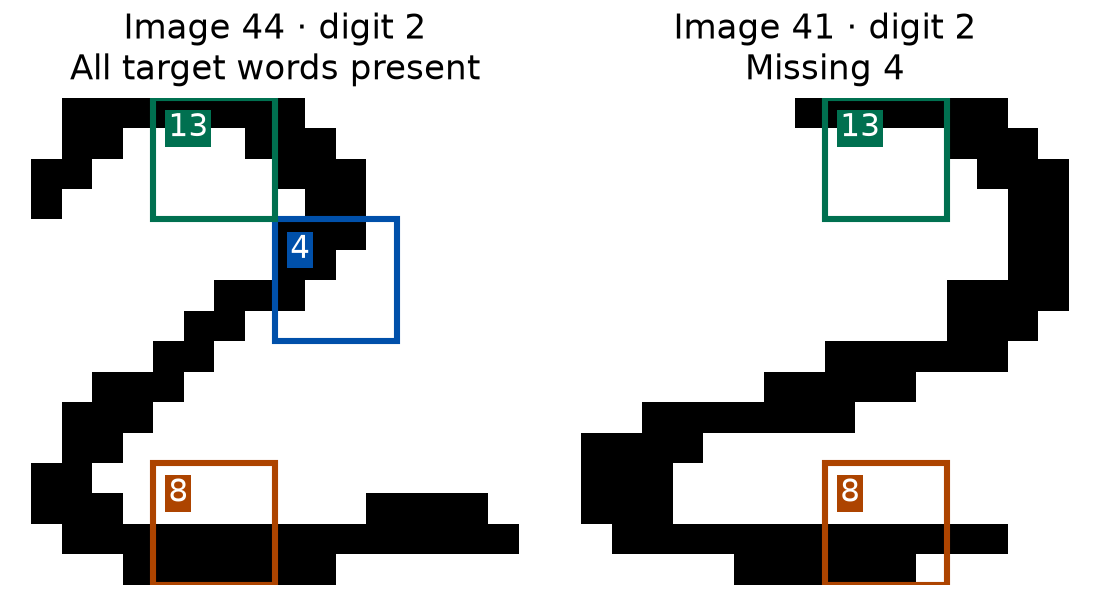
\includegraphics[width=\columnwidth]{figures/semeion-source-contrast.png}
\caption{Two source images, both labeled as the digit 2. The boxes mark patches assigned to
the corresponding words. Image 44 contains the full triple $\{4,8,13\}$. Image 41 lacks
word 4.}
\label{fig:semeion-contrast}
\end{figure}

\subsubsection{Sensitivity to codebook size and minsup}
Table~\ref{tab:semeion-sensitivity} compares itemset counts across codebook size $K$ and
minsup, with the same seed, patch grid, maximum iterations, and distance threshold. Empty
images are images with no patch assigned to a word. With $K=24$, word 13 and the pair
$\{8,13\}$ reach all five thresholds. The triple $\{4,8,13\}$ has support 90, which reaches
the 5.5\% threshold (88 images) and falls below the 6\% threshold (96 images).

\begin{table}[t]
\centering
\caption{Itemset counts by codebook size $K$ and minsup on Semeion}
\label{tab:semeion-sensitivity}
\begin{tabular}{rrrrrrr}
\hline
$K$ & Empty images & 20\% & 10\% & 6\% & 5.5\% & 5\% \\
\hline
16 & 99 & 4 & 12 & 19 & 21 & 25 \\
24 & 11 & 6 & 18 & 35 & 43 & 46 \\
32 & 2 & 5 & 24 & 45 & 52 & 63 \\
\hline
\end{tabular}
\end{table}

As $K$ grows from 16 to 32, the mean width grows from 2.27 to 4.31 words per image. At the
20\% threshold, the 24-word codebook gives the most patterns of the three configurations.
The centers are learned again for each $K$, so the representative patches need comparing
before a word is interpreted across configurations. How frequent a stroke is also depends
on where the grid falls and on the resolution of the binary image.

\subsubsection{Uses and limitations}
Visual patterns can serve as queries by stroke combination. For example, the query
$\{8,13\}$ returns 330 images. Normalized by the number of images per label, this pattern
appears in 69 of 159 images of the digit 3 (43.4\%) and 9 of 161 images of the digit 4
(5.6\%). The gap describes label frequencies in the same dataset used to learn the
codebook. The two words can appear at any position in the image.

Each itemset can also define a binary feature. With the pattern list
$(\{13\},\{8,13\},\{4,8,13\})$, an image with transaction $\{8,13\}$ gets the vector
$(1,1,0)$. The notebook builds a matrix with 1\,593 image rows and 46 itemset columns at
minsup 5\%. Each column sums to the support of its itemset. To evaluate these features for
classification, the codebook and the patterns would have to be learned on a training set
and then held fixed while encoding the test set. The analysis here describes frequencies
on Semeion.

The \href{https://github.com/NgTHung/Itemset/blob/main/notebooks/image_patterns_colab.ipynb}
{image-pattern notebook} uses Julia 1.13.2 and seed 42 to reproduce the default pipeline.
The run manifest records the revision, the seed, and the hashes of the codebook and the
outputs at minsup 20\%, 10\%, and 5\%. The grid in Table~\ref{tab:semeion-sensitivity}
uses the same encoder in 15 configurations.

\section{Conclusion}
We implemented Eclat from the original paper~\cite{zaki2000} as two variants that return
the same result. Both match SPMF's Eclat exactly at every database and threshold, with 66
comparisons over 33 pairs and no missing, extra, duplicate, or wrong-support itemset
(Section~\ref{sec:exact-memory}). In a single timing session on the grading machine, the
optimized variant is the fastest at all 33 points. At the lowest minsup of each database
it is 7.9 times (Accidents) to 33.3 times (Retail) faster than the baseline
(Section~\ref{sec:minsup}), and Section~\ref{sec:optimized} breaks the gain down by
optimization step. The baseline's time tracks the total length of the tidsets it merges,
at 2.0 to 6.9\,ns per element. When transaction length grows from 5 to 40 with output held
fixed, the baseline's mining time grows 53-fold while the optimized variant's grows only
1.8-fold (Section~\ref{sec:width}). The optimized variant's peak memory is 11.0\% to
34.4\% lower than the baseline's at the mid-range threshold of each database
(Section~\ref{sec:exact-memory}).

Both applications use the same miner. On the 39\,516 invoices of Online Retail II, minsup
0.01 gives 1\,355 frequent itemsets, from which we generate association rules and rank them
by lift (Section~\ref{sec:basket}). On the 1\,593 Semeion images, a 24-word visual
codebook turns each image into a transaction, and the frequent itemsets describe stroke
combinations that recur across images (Section~\ref{sec:visual-patterns}).

The conclusions have limits. Runtime was measured on one grading machine, while
transaction length and memory were measured on two other Windows machines, so programs
should be compared only within the same session. The \emph{process} scope includes Julia
or JVM start-up, so at high thresholds, where the two Julia variants are close, start-up
is most of the time. We treat SPMF as a black box, so we do not explain the differences
we measured in terms of SPMF's internals. The basket data comes from a single
shop over two years, and the image patterns describe frequencies within the same set used
to learn the codebook, so they say nothing yet about classification accuracy.

Two next steps follow from the optimized variant's time profile (Section~\ref{sec:future}):
a flat integer store with an array-built vertical layout, to cut the reading and layout
time that takes almost the whole run on Accidents, and output in search order, to drop the
sort that takes 28\% to 37\% of the run at the dense points. Both are predictions with a
plan for testing them, and neither has been implemented.

\bibliographystyle{IEEEtran}
\bibliography{references}
\end{document}
